\section{Tổng và hiệu của hai vectơ}

\subsection{TÓM TẮT LÝ THUYẾT}
\subsubsection{Phép toán cộng hai vectơ}
Phép cộng hai vectơ có tính chất giao hoán. Khi thực hiện phép toán cộng hai vectơ, ta chú ý các quy tắc sau
\begin{itemize}
	\item [\iconMT] \indamm{Quy tắc 3 điểm:} ("nối đuôi")
	\immini[thm]{Với ba điểm $A,B,C$ bất kì, ta luôn có
		\fbox{$\overrightarrow{AB}+\overrightarrow{BC}=\overrightarrow{AC}$}
		
	}{
	\begin{tikzpicture}[scale=0.6, line join=round, line cap=round]
	\tkzDefPoints{0/0/A,5/0/C,2/2/B}
	\tkzDrawSegments(A,B B,C C,A)
	\tkzDrawPoints[size=2,fill=black](A,B,C)
	\tkzLabelPoints[above](B)
	\tkzLabelPoints[below](A,C)
	\end{tikzpicture}}

	\item [\iconMT] \indamm{Quy tắc hình bình hành:} ("chung đầu")
	% \begin{boxkn}
	\immini[thm]{Xét hình bình hành $ABCD$, ta luôn có
		\fbox{$\overrightarrow{AB}+\overrightarrow{AD}=\overrightarrow{AC}$}
		
	}{
		\begin{tikzpicture}[scale=0.6, line join=round, line cap=round]
		\tkzDefPoints{0/0/A,1/2/B,5/2/C,4/0/D}
		\tkzDrawSegments(A,B B,C C,D D,A)
		\tkzDrawPoints[size=2,fill=black](A,B,C,D)
		\tkzLabelPoints[below](A,D)
		\tkzLabelPoints[above](B,C)
		\end{tikzpicture}}
	\item [\iconMT] \indamm{Quy tắc cộng vectơ đối:} Nếu $\overrightarrow{a}$ và $\overrightarrow{b}$ đối nhau thì $\overrightarrow{a}+\overrightarrow{b}=\overrightarrow{0}$.
\end{itemize}
\indamm{Tính chất:} Với ba vectơ $\vec{a}$, $\vec{b}$, $\vec{c}$ tùy ý
\begin{tcolorbox}[colframe=orange,colback=white,boxrule=0.2mm]
	\begin{itemize}
		\item Tính chất giao hoán: $\vec{a}+\vec{b}=\vec{b}+\vec{a}$.
		\item Tính chất kết hợp: $(\vec{a}+\vec{b})+\vec{c}=\vec{a}+(\vec{b}+\vec{c})$.
		\item Tính chất của vectơ-không: $\vec{a}+\vec{0}=\vec{a}$.
	\end{itemize}
\end{tcolorbox}

\subsubsection{Phép toán hiệu hai vectơ}
	\begin{itemize}
		\item [\iconMT] \indamm{Vectơ đối:} 
		\begin{itemize}
			\item [$\bullet$] Vectơ đối của $\vec{a}$ kí hiệu là $-\vec{a}$.
			\item [$\bullet$] Vectơ đối của $\overrightarrow{AB}$ là $\overrightarrow{BA}$, nghĩa là \fbox{$-\overrightarrow{AB}=\overrightarrow{BA}$} (\textit{dùng để làm mất dấu trừ trước vectơ}).
			\item [$\bullet$] Vectơ $\vec{0}$ được coi là vectơ đối của chính nó.
		\end{itemize} 
		\item [\iconMT] \indamm{ Quy tắc trừ:} Với ba điểm $A,B,C$ bất kì, ta luôn có
		\fbox{$\overrightarrow{BC}=\overrightarrow{AC}-\overrightarrow{AB}$}
	\end{itemize}
\subsubsection{Công thức trung điểm, trọng tâm}
\begin{itemize}
	\item [\iconMT] \indamm{Công thức trung điểm:} Nếu $M$ là trung điểm của đoạn $AB$ thì $$\overrightarrow{MA}+\overrightarrow{MB}=\overrightarrow{0}$$
	\begin{center}
		\begin{tikzpicture}[scale=1, line join=round, line cap=round]
		\tikzset{label style/.style={font=\footnotesize}}
		\tkzDefPoints{0/0/A,4/0/B}
		\coordinate (M) at ($(A)!0.5!(B)$);
		\tkzDrawPoints[size=2,fill=black](A,B,M)
		\tkzDrawSegments(A,B)
		\tkzLabelPoints[above](A,B,M)	
\end{tikzpicture}
	\end{center}
	\item [\iconMT] \indamm{Công thức trọng tâm:} Nếu $G$ là trọng tâm của tam giác $ABC$ thì $$\overrightarrow{GA}+\overrightarrow{GB}+\overrightarrow{GC}=\overrightarrow{0}.$$
\begin{center}
	\begin{tikzpicture}[scale=1, line join=round, line cap=round]
		\tikzset{label style/.style={font=\footnotesize}}
		\tkzDefPoints{0/0/B,4/0/C,1/2/A}
		\coordinate (I) at ($(C)!0.5!(B)$);
		\coordinate (K) at ($(A)!0.5!(B)$);
		\coordinate (M) at ($(C)!0.5!(A)$);
		\tkzInterLL(A,I)(C,K)\tkzGetPoint{G}
		\tkzDrawSegments(A,B B,C C,A A,I C,K B,M)
		\tkzDrawPoints[size=2,fill=black](A,B,C,I,K,M,G)
		\tkzLabelPoints[below](C, B,I)
		\tkzLabelPoints[above](A)
		\tkzLabelPoints[above right](M)
		\tkzLabelPoints[above left](K)
		\tkzLabelPoints[above right](G)
\end{tikzpicture}
\end{center}
\end{itemize}
\subsection{Các dạng toán}
\setcounter{dang}{0}
\begin{dang}{Tính tổng, hiệu hai vectơ}
	%{\bf Quy tắc 1. Lập bảng biến thiên suy ra kết luận về cực trị}
	\begin{itemize}
		\item Ghép các vectơ lại thích hợp. 
		\item Dùng các quy tắc cộng vectơ để tính. 
	\end{itemize}
\end{dang}
\viduminhhoa
\begin{vd}
	\immini[thm]{Cho tam giác $ABC$. Các điểm $M$, $N$ và $K$ lần lượt là trung điểm của $AB$, $AC$ và $BC$.
	\begin{tasks}(1)
		\task Tìm các vectơ bằng với $\overrightarrow{MK}$.
		\task Tìm các vectơ đối của $\overrightarrow{MN}$.
		\task  Xác định các vectơ $\overrightarrow{AM}+\overrightarrow{MN}$;\quad $\overrightarrow{AM}+\overrightarrow{NK}$;\quad $\overrightarrow{AM}+\overrightarrow{KN}$;\quad $\overrightarrow{AM}-\overrightarrow{AN}$; \quad $\overrightarrow{MN}-\overrightarrow{NC}$;\quad $\overrightarrow{BK}-\overrightarrow{CK}$.
	\end{tasks}}{
		\begin{tikzpicture}[scale=1, line join=round, line cap=round]
	\tkzDefPoints{0/0/A,1/2/B,4/0/C}
	\coordinate (M) at ($(A)!0.5!(B)$);
	\coordinate (N) at ($(C)!0.5!(A)$);
	\coordinate (K) at ($(B)!0.5!(C)$);
	\tkzDrawSegments(A,B B,C C,A)
	\tkzDrawPoints[size=2,fill=black](A,B,C,M,N,K)
	\tkzLabelPoints[below, font=\footnotesize](A,N,C)
	\tkzLabelPoints[above, font=\footnotesize](B)
	\tkzLabelPoints[above left, font=\footnotesize](M)
	\tkzLabelPoints[above right, font=\footnotesize](K)
	\end{tikzpicture}}
	
\end{vd}

\begin{vd}
	\immini[thm]{Cho hình bình hành $ABCD$ tâm $O$. 
		\begin{tasks}(1)
			\task Tìm  vectơ bằng với $\overrightarrow{OC}$.
			\task Xác định các vectơ $\overrightarrow{OA}+\overrightarrow{OC}$;\quad $\overrightarrow{OB}+\overrightarrow{OD}$;\quad $\overrightarrow{AB}+\overrightarrow{CD}$;\quad $\overrightarrow{AD}-\overrightarrow{BC}$;\quad $\overrightarrow{OA}+\overrightarrow{DC}$ .
		\end{tasks}
}{
		\begin{tikzpicture}[scale=1, line join=round, line cap=round]
	\tkzDefPoints{0/0/A,1/2/B,5/2/C,4/0/D}
	\tkzInterLL(A,C)(B,D)\tkzGetPoint{O}
	\tkzDrawSegments(A,B B,C C,D D,A A,C B,D)
	\tkzDrawPoints[size=2,fill=black](A,B,C,D,O)
	\tkzLabelPoints[below, font=\footnotesize](A,D)
	\tkzLabelPoints[above, font=\footnotesize](B,C,O)
	\end{tikzpicture}}

\end{vd}


\begin{vd}
\immini[thm]{Cho hình bình hành $ABCD$ Hai điểm $M$ và $N$ lần lượt là trung điểm của $BC$ và $AD$ Xác định vectơ
	\begin{listEX}[2]
		\item [] $\overrightarrow{DA}+\overrightarrow{DC}$,
		\item [] $\overrightarrow{AM}+\overrightarrow{AN}$,
		\item [] $\overrightarrow{AN}+\overrightarrow{CM}$,
		\item [] $\overrightarrow{MB}+\overrightarrow{NC}$.
	\end{listEX}    
}{
		\begin{tikzpicture}[scale=0.9, line join=round, line cap=round]
	\tkzDefPoints{0/0/A,1/2/B,5/2/C,4/0/D}
	\coordinate (M) at ($(C)!0.5!(B)$);
	\coordinate (N) at ($(A)!0.5!(D)$);
	\tkzDrawSegments(A,B B,C C,D D,A M,N)
	\tkzDrawPoints[size=2,fill=black](A,B,C,D,M,N)
	\tkzLabelPoints[below, font=\footnotesize](A,D,N)
	\tkzLabelPoints[above, font=\footnotesize](B,C,M)
	\end{tikzpicture}}
\end{vd}

\baitaptl

\begin{bt}%[BG1-2022-Huỳnh Xuân Tín]%[0H1Y2-1]
	Tính tổng $\overrightarrow{MN}+\overrightarrow{PQ}+\overrightarrow{RN}+\overrightarrow{NP}+\overrightarrow{QR}$.
	\loigiai{
		Ta có $\overrightarrow{MN}+\overrightarrow{PQ}+\overrightarrow{RN}+\overrightarrow{NP}+\overrightarrow{QR}=\overrightarrow{MN}+\overrightarrow{NP}+\overrightarrow{PQ}+\overrightarrow{QR}+\overrightarrow{RN}=\overrightarrow{MN}$.
	}
\end{bt}

\begin{bt}%[BG1-2022-Huỳnh Xuân Tín]%[0H1B2-2]
	Cho tam giác $ABC$ với $M$, $ N$, $ P$ lần lượt là trung điểm của $BC$, $ CA$, $ AB$. Tính tổng $\overrightarrow{AP}+\overrightarrow{BM}+\overrightarrow{CN}$.
	\loigiai{
		\immini[thm]{Dễ dàng có $BPNM$ là  hình bình hành suy ra 	$\overrightarrow{BM}=\overrightarrow{PN}$ và $\overrightarrow{CN}=\overrightarrow{NA}$ vì $N$ là  trung điểm của $CA$. Do đó
			$$\overrightarrow{AP}+\overrightarrow{BM}+\overrightarrow{CN}=\overrightarrow{AP}+\overrightarrow{PN}+\overrightarrow{NA}=\overrightarrow{0}.$$}
		{\begin{tikzpicture}[scale=0.7, font=\footnotesize, line join = round, line cap = round,>=stealth]
				\tkzDefPoints{0/0/A, 6/0/B,2/4/C}
				\tkzDefMidPoint(A,B) \tkzGetPoint{P}
				\tkzDefMidPoint(A,C) \tkzGetPoint{N}
				\tkzDefMidPoint(B,C) \tkzGetPoint{M}	
				\tkzDrawPoints[fill=black](A,B,C,M,N,P)
				\tkzDrawPolygon(A,B,C)
				\tkzDrawPolygon(M,N,P)
				\tkzLabelPoints[above](C) 
				\tkzLabelPoints[below](B,A,P)
				\tkzLabelPoints[left](N)
				\tkzLabelPoints[right](M)
		\end{tikzpicture}}
	}
\end{bt}

\begin{bt}%[BG1-2022-Huỳnh Xuân Tín]%[0H1K2-1]
	Cho hai hình bình hành $ ABCD $ và $ AB'C'D' $ có chung đỉnh $ A $. Tính  $\vec{u}= \vec{B'B}  + \vec{CC'}  + \vec{D'D}$.
	\loigiai{
		Theo quy tắc trừ và quy tắc hình bình hành ta có
		\begin{eqnarray*}
			\vec{B'B}  + \vec{CC'}  + \vec{D'D}&=&(\vec{AB}  - \vec{AB'}) + (\vec{AC'}  - \vec{AC}) + (\vec{AD}  - \vec{AD'})\\
			&=&(\vec{AB}  + \vec{AD}) - \vec{AC}  - (\vec{AB'}  + \vec{AD} ') + \vec{AC}\\
			&=& \overrightarrow{0}
		\end{eqnarray*}
		Vậy $\vec{u}=0$.
	}
\end{bt}

\begin{bt}%[BG1-2022-Huỳnh Xuân Tín]%[0H1K2-1] 
	Cho tam giác $ABC$, gọi $D,E,F$, $G,H,I$ theo thứ tự là trung điểm các cạnh $AB,BC,CA$,
	$DF,DE,EF$. Tính vectơ $\vec{u} =\vec{BE}-\vec{GH} -\vec{AI}+\vec{FE}$?
	\loigiai{
		\immini[thm]{
			Ta có
			\begin{eqnarray*}
				\vec{u}&=&\vec{BE}-\vec{GH} -\vec{AI}+\vec{FE}\\
				&=&\left(\vec{BE}+\vec{FE}\right)-\left(\vec{GH}+\vec{AI}\right)\\
				&=&\left(\vec{BE}+\vec{FE}\right)-\left(\vec{IE}+\vec{AI}\right)\\
				&=&\vec{DE}-\vec{AE}=\vec{DA}.
			\end{eqnarray*}
		}
		{
			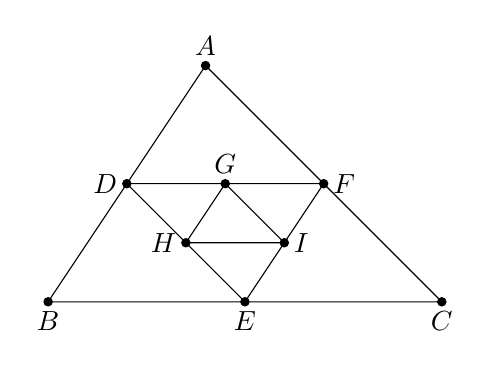
\begin{tikzpicture}
				\coordinate (A) at (0,2); \coordinate (B) at (-2,-1); \coordinate (C) at (3,-1); 
				\coordinate (D) at (-1,0.5); \coordinate (E) at (0.5,-1); \coordinate (F) at (1.5,0.5); 
				\coordinate (G) at (0.25,0.5); \coordinate (H) at (-0.25,-0.25); \coordinate (I) at (1,-0.25); 
				\draw (A)--(B)--(C)--(F)--(E)--(D)--(G)--(H)--(I)--(G)--(F)--(A);
				\foreach \i in {B,E,C} \draw[fill]  (\i) circle (1.5pt) node[below] {$\i$}; 
				\foreach \i in {A,G} \draw[fill]  (\i) circle (1.5pt) node[above] {$\i$}; 
				\foreach \i in {D,H} \draw[fill]  (\i) circle (1.5pt) node[left] {$\i$}; 
				\foreach \i in {I,F} \draw[fill]  (\i) circle (1.5pt) node[right] {$\i$}; 
			\end{tikzpicture}
		}
	}
\end{bt}


\begin{bt}%[[BG1-2022-Huỳnh Xuân Tín]%[0H1K2-1]
	\immini[thm]{Cho lục giác đều $ABCDEF$ tâm $O$. Rút gọn vectơ $\vec{v} =\vec{AF}+\vec{BC}+\vec{DE}$?
	}
	{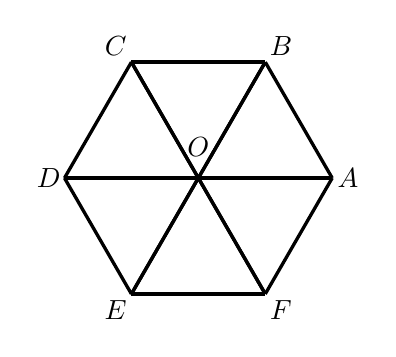
\begin{tikzpicture}[scale=1.7,very thick]
			\foreach \x in {0,60,...,300} {
				\draw (\x:1 cm) -- (\x + 60:1 cm);
				\draw (\x:1 cm) -- (\x + 180:1 cm);
			}
			\draw  (0:1 cm) node[shift={(0.2,0)}] {$A$}; \draw  (60:1 cm) node[shift={(0.2,0.2)}] {$B$}; 
			\draw  (120:1 cm) node[shift={(-0.2,0.2)}] {$C$}; \draw  (180:1 cm) node[shift={(-0.2,0)}] {$D$}; 
			\draw  (240:1 cm) node[shift={(-0.2,-0.2)}] {$E$}; \draw  (300:1 cm) node[shift={(0.2,-0.2)}] {$F$}; 
			\draw  (0,0.08 ) node[above] {$O$}; 
	\end{tikzpicture}}
	\loigiai{
		$\vec{v} =\vec{AF}+\vec{BC}+\vec{DE}=\vec{BO}+\vec{BC}+\vec{CO}=\vec{BO}+\vec{BO}=\vec{BO}+\vec{OE}=\vec{BE}.$
	}
\end{bt}

\begin{bt}%[BG1-2022-Huỳnh Xuân Tín]%[0H1K2-1]
	Gọi $O$ là tâm của tam giác đều $ABC$. Tính $\vec{u}=\overrightarrow{OA}+\overrightarrow{OB}+\overrightarrow{OC}$.
	\loigiai{
		\immini[thm]{Vẽ lục giác đều $AMBNCP$ nội tiếp đường tròn $(O)$. \\
			Vì $BOCN$ là hình bình hành nên $\overrightarrow{OB}+\overrightarrow{OC}=\overrightarrow{ON}$. \\
			Do đó $\vec{u}=\overrightarrow{OA}+\overrightarrow{OB}+\overrightarrow{OC}=\overrightarrow{OA}+\overrightarrow{ON}=\overrightarrow{0}$.}
		{\begin{tikzpicture}[scale=1.4]
				\def \r{1}\def \x{60} \tkzDefPoints{0/0/O}
				\coordinate (A) at (0*\x:\r);
				\coordinate (M) at (1*\x:\r);
				\coordinate (B) at (2*\x:\r);
				\coordinate (N) at (3*\x:\r);
				\coordinate (C) at (4*\x:\r);
				\coordinate (P) at (5*\x:\r);
				\draw (O) circle(\r cm);
				\tkzDrawPoints[fill=black](O,A,B,C,M,N,P)
				\tkzDrawPolygon(A,M,B,N,C,P,A,B,C)
				\tkzDrawSegments(M,C B,P A,N)
				\tkzLabelPoints[left](N)
				\tkzLabelPoints[right](A)
				\tkzLabelPoints[below](C,P)
				\tkzLabelPoints[above](M,B)
	\end{tikzpicture}}}
\end{bt}

\begin{bt}%[BG1-2022-Huỳnh Xuân Tín]%[0H1K2-1]
	Cho hình bình hành $ABCD$. Trên các đoạn thẳng $DC,AB$ theo thứ tự lấy các điểm $M,N$ sao cho $DM=BN$. Gọi $P$ là giao điểm của $AM,DB$ và $Q$ là giao điểm của $CN,DB$. Tính $\vec{u}=\overrightarrow{DP}-\overrightarrow{QB}$.
	\loigiai{
		Ta có $DM=BN \Rightarrow AN=MC$, mặt khác $AN$ song song với $MC$ do đó tứ giác $ANCM$ là
		\immini[thm]{
			hình bình hành. Suy ra $\overrightarrow{AM}=\overrightarrow{NC}$.\\
			Xét tam giác $\triangle DMP$ và $\triangle BNQ$ ta có\\
			\indent\qquad\qquad
			$\left\{\begin{aligned}
				&DM=NB\text{ (giả thiết)}\\
				&\widehat{PDM}=\widehat{QBN} \text{ (so le trong)}.\\
			\end{aligned}\right.$}
		{\begin{tikzpicture}[scale=1,>=stealth, line join=round, line cap=round]
				\tkzDefPoints{0/0/A,5/0/B,3.5/-2/C}
				\coordinate (D) at ($(A)+(C)-(B)$);
				\coordinate (M) at ($(D)!1/3!(C)$);
				\coordinate (N) at ($(A)+(C)-(M)$);
				\tkzInterLL(A,M)(B,D)\tkzGetPoint{P}
				\tkzInterLL(C,N)(B,D)\tkzGetPoint{Q}
				\tkzDrawPolygon(A,B,C,D)
				\tkzDrawSegments(B,D A,M C,N)
				\tkzDrawPoints[fill=black](A,B,C,D,M,N,P,Q)
				\tkzLabelPoints[below](D,M,C)
				\tkzLabelPoints[above](A,N,B)
				\tkzLabelPoints[above left](P)
				\tkzLabelPoints[below right](Q)
		\end{tikzpicture}}
		\noindent
		Mặt khác $\widehat{DMP}=\widehat{APB}$ (đối đỉnh) và $\widehat{APQ}=\widehat{NQB}$ (hai góc đồng vị) suy ra $\widehat{DMP}=\widehat{BNQ}$.\\
		Do đó $\triangle DMP=\triangle BNQ$ (c.g.c) suy ra $DB=QB$.\\
		Dễ thấy $\overrightarrow{DP},\overrightarrow{QB}$ cùng hướng vì vậy $\overrightarrow{DP}=\overrightarrow{QB}$ hay $\vec{u}=\overrightarrow{DP}-\overrightarrow{QB}=0$.}
\end{bt}


% \begin{bt}%[BG1-2022-Huỳnh Xuân Tín]%[0H1B2-1]
% 	Cho tam giác $ABC$ đều, $G$ là trọng tâm, tính $\vec{GB}+\vec{GC}$.
% 	\loigiai{		
% 		\immini[thm]{	
% 			Dựng hình bình hành $GBOC$.
% 			Ta có: $\vec{GB}+\vec{GC}=\vec{GO}$.
% 		}{	\begin{tikzpicture}[>=stealth,scale=.7]
% 				\tkzDefPoints{0/0/B,5/0/C}
% 				\tkzDefMidPoint(B,C)\tkzGetPoint{M}
% 				\tkzDefTriangle[equilateral](B,C)\tkzGetPoint{A}
% 				\tkzDefPointWith[linear,K=.66](A,M)\tkzGetPoint{G}
% 				\tkzDefPointBy[translation=from G to M](M)\tkzGetPoint{O}
% 				\tkzDrawSegments[](A,B B,C C,A A,M B,O B,C O,C)
% 				\tkzDrawVectors[>=stealth](G,C G,B G,O)
% 				\tkzLabelPoints[above](A)	\tkzLabelPoints[left](B)
% 				\tkzLabelPoints[right](G,C)
% 				\tkzLabelPoints[below](O)
% 				\tkzDrawPoints(A,B,G,C,O) 
% 			\end{tikzpicture}
% 		}
% 	}
% \end{bt}

% \begin{bt}%[BG1-2022-Huỳnh Xuân Tín]%[0H1B2-1]
% 	Cho tam giác $ABC$ đều, $G$ là trọng tâm, tính $\vec{AG}+\vec{CB}$.
% 	\loigiai{
% 		\immini[thm]{	
% 			Ta có: $\vec{AG}+\vec{CB}=\vec{BF}+\vec{CB}=\vec{CF}$ (dựng $\vec{BF}=\vec{AG}$).
% 		}{	
% 			\begin{tikzpicture}[>=stealth,scale=.6]
% 				\tkzDefPoints{0/0/B,5/0/C}%,8/4/B,13/0/C}
% 				\tkzDefMidPoint(B,C)\tkzGetPoint{M}
% 				\tkzDefTriangle[equilateral](B,C)\tkzGetPoint{A}
% 				\tkzDefPointWith[linear,K=.66](A,M)\tkzGetPoint{G}
% 				\tkzDefPointBy[translation=from A to G](B)\tkzGetPoint{F}
% 				\tkzDrawSegments[](A,B B,C C,A A,M)
% 				\tkzDrawVectors[>=stealth](A,G A,B B,F A,F)
% 				\tkzLabelPoints[above](A)	\tkzLabelPoints[left](B)
% 				\tkzLabelPoints[right](G,C)
% 				\tkzLabelPoints[below](F)
% 				\tkzDrawPoints(A,B,G,C,F) 
% 				%\tkzLabelPoints[right](C,B)
% 			\end{tikzpicture}
% 		}
% 	}
% \end{bt}


\begin{dang}{Xác định vị trí của một điểm từ đẳng thức vectơ}
\end{dang}
	\viduminhhoa
	\begin{vd}%[Dự án Bài giảng Toán 10 (2022)]%[Kiều Ngân]%[0H1B2-3]
		Cho tam giác $ABC$. Điểm $M$ thỏa mãn điều kiện $\overrightarrow{MA}+\overrightarrow{MB}+\overrightarrow{MC}=\overrightarrow{0}$. Mệnh đề nào sau đây đúng?
		\choice
		{$M$ là điểm sao cho tứ giác $BAMC$ là hình bình hành}
		{$M$ là điểm sao cho tứ giác $ABMC$ là hình bình hành}
		{\True $M$ là trọng tâm tam giác $ABC$}
		{$M$ thuộc đường trung trực của $AB$}
		\loigiai{
			Ta có $\overrightarrow{MA}+\overrightarrow{MB}+\overrightarrow{MC}=\overrightarrow{0}$ nên $M$ là trọng tâm tam giác $ABC$.
		}
	\end{vd} 
	\baitaptl   
	\begin{bt}%[Dự án Bài giảng Toán 10 (2022)]%[Kiều Ngân]%[0H1B2-3]
		Cho tam giác $ABC$. Xác định điểm $M$ thỏa mãn điều kiện $\overrightarrow{MA}-\overrightarrow{MB}+\overrightarrow{MC}=\overrightarrow{0}$. 
		% Mệnh đề nào sau đây đúng?
		% \choice
		% {$M$ thuộc trung trực của $AB$}
		% {$M$ là trọng tâm tam giác $ABC$}
		% {\True $M$ là điểm sao cho tứ giác $BAMC$ là hình bình hành}
		% {$M$ là điểm sao cho tứ giác $ABMC$ là hình bình hành}
		\loigiai{
			Ta có $\overrightarrow{MA}-\overrightarrow{MB}+\overrightarrow{MC}=\overrightarrow{0}\Leftrightarrow
			\overrightarrow{MA}-\overrightarrow{MB}=-\overrightarrow{MC}\Leftrightarrow \overrightarrow{BA}=\overrightarrow{CM}$.\\\
			Suy ra $M$ là đỉnh của hình bình hành $BAMC$.
		}
	\end{bt}
	\begin{bt}%[Dự án Bài giảng Toán 10 (2022)]%[Kiều Ngân]%[0H1B2-3]
		Cho hình bình hành $ABCD$. Xác định điểm $M$ thỏa mãn điều kiện $\overrightarrow{AB}+\overrightarrow{AC}+\overrightarrow{AD}=\overrightarrow{AM}$. 
		% Khẳng định nào sau đây đúng?
		% \choice
		% {\True $M$ đối xứng với $A$ qua $C$}
		% {$M$ đối xứng với $B$ qua $C$}
		% {$M$ đối xứng với $D$ qua $C$}
		% {$M$ trùng với điểm $C$}
		\loigiai{
			Vì $ABCD$ là hình bình hành nên $\overrightarrow{AB}+\overrightarrow{AD}=\overrightarrow{AC}$.\\
			Khi đó $\overrightarrow{AB}+\overrightarrow{AC}+\overrightarrow{AD}=\overrightarrow{AM}\Leftrightarrow
			\overrightarrow{AB}+\overrightarrow{AD}=\overrightarrow{AM}-\overrightarrow{AC}\Leftrightarrow \overrightarrow{AC}=\overrightarrow{CM}$.\\\
			Suy ra $M$ đối xứng với $A$ qua $C$.
		}
	\end{bt}
	\begin{bt}%[Dự án Bài giảng Toán 10 (2022)]%[Kiều Ngân]%[0H1B2-3]
		Cho hình bình hành $ABCD$. Xác định điểm $M$ thỏa mãn điều kiện $\left|\overrightarrow{MB}+\overrightarrow{CD}\right|=\left|\overrightarrow{MC}+\overrightarrow{DA}\right|$.
		% Khẳng định nào sau đây đúng?
		% \choice
		% {\True $M$ thuộc đường trung trực của cạnh $AB$}
		% {$M$ là trung điểm $AB$}
		% {$M$ là trung điểm $CD$}
		% {$M$ thuộc đường trung trực của cạnh $CD$}
		\loigiai{
			\immini[thm]{
				Vì $ABCD$ là hình bình hành nên $\heva{&\overrightarrow{BA}=\overrightarrow{CD}\\&\overrightarrow{DA}=\overrightarrow{CB}.}$\\
				Ta có
				\allowdisplaybreaks
				\begin{eqnarray*}
					&&\left|\overrightarrow{MB}+\overrightarrow{CD}\right|=\left|\overrightarrow{MC}+\overrightarrow{DA}\right|\\
					&\Leftrightarrow&\left|\overrightarrow{MB}+\overrightarrow{BA}\right|=\left|\overrightarrow{MC}+\overrightarrow{CB}\right|\\
					&\Leftrightarrow&\left|\overrightarrow{MA}\right|=\left|\overrightarrow{MB}\right|\Leftrightarrow MA=MB.
				\end{eqnarray*}
				Vậy $M$ thuộc đường trung trực của cạnh $AB$.
			}{
				\begin{tikzpicture}[scale=1, font=\footnotesize, line join=round, line cap=round, >=stealth]
					\path
					(0,0) coordinate (A)
					(2.8,0) coordinate (B)
					(-0.8,-1.2) coordinate (D)
					($(B)+(D)-(A)$) coordinate (C)
					;
					\draw (A)--(B)--(C)--(D)--(A);
					\foreach \x/\g in {A/130,B/30,C/-60,D/-145} \draw[fill=black] (\x) circle(1pt) +(\g:0.3) node{$\x$};
				\end{tikzpicture}
			}
		}
	\end{bt}	


\begin{dang}{Tính độ dài vectơ}
	
\end{dang}
\viduminhhoa
\begin{vd}%[Phan Anh]%[Dự án giáo án 10]%[0H1B2-5]
	Cho tam giác đều $ABC$ có cạnh $AB=a$, xác định và tính độ dài của vectơ
	\begin{enumEX}{2}
		\item $\overrightarrow{x}=\overrightarrow{AB}+\overrightarrow{BC}$.
		\dapso{$a$.}
		\item $\overrightarrow{y}=\overrightarrow{AB}+\overrightarrow{AC}$.
		\dapso{$a\sqrt{3}$.}
	\end{enumEX}
	\loigiai{\begin{center}
			\begin{tikzpicture}[>=stealth,line join=round,line cap=round,font=\footnotesize,scale=0.7]
				\path (0,0) coordinate (A)
				(2,{2*sqrt(3)}) coordinate (B)
				(4,0) coordinate (C)
				($(B)+(C)-(A)$) coordinate (D)
				($(B)!0.5!(C)$) coordinate (M)
				;
				\draw (A)--(B)--(C)--(A) (B)--(D)--(A);
				\foreach\p /\r in {A/-135,B/90,C/-45,D/45,M/70}
				\fill (\p) circle (1.2pt) node[shift={(\r:3mm)}]{$\p$};
			\end{tikzpicture}
		\end{center}
		\begin{enumerate}
			\item Ta có $\overrightarrow{x}=\overrightarrow{AB}+\overrightarrow{BC}=\overrightarrow{AC}$.\\
			Suy ra $\left|\overrightarrow{x}\right|=\left|\overrightarrow{AC}\right|=AC=a$.
			\item Dựng $\overrightarrow{BD}=\overrightarrow{AC}$, ta có $\overrightarrow{y}=\overrightarrow{AB}+\overrightarrow{AC}=\overrightarrow{AB}+\overrightarrow{BD}=\overrightarrow{AD}$.\\
			Suy ra $\left|\overrightarrow{y}\right|=\left|\overrightarrow{AD}\right|=AD$.\\
			Gọi $M$ là trung điểm của $BC$, ta có $AD=2AM=2\cdot\dfrac{a\sqrt{3}}{2}=a\sqrt{3}$. Vậy $\left|\overrightarrow{y}\right|=a\sqrt{3}$.
	\end{enumerate}}
\end{vd}
\begin{vd}
\immini{Cho hình vuông $ABCD$ tâm $O$ cạnh bằng $a$. Tính 
	\begin{tasks}(3)
		\task $\left| \overrightarrow{AB}+\overrightarrow{BC} \right|$.
		\task $\left| \overrightarrow{AB}-\overrightarrow{AC} \right|$.
		\task $\left|\vec{AB}+\vec{OD} -\vec{BC}\right|$.
	\end{tasks}}{
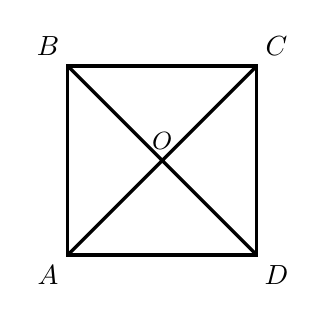
\begin{tikzpicture}[very thick,scale=1.2]
	\coordinate (M) at (0,0); \coordinate (N) at (2,0); \coordinate (P) at (2,2);
	\coordinate (Q) at (0,2); \coordinate (O) at (1,1);
	\draw (M)--(N)--(P)--(Q)--cycle; \draw (M)--(P) (N)--(Q);
	\draw (M) node[shift={(-0.25,-0.25)}] {$A$};
	\draw (Q)  node[shift={(-0.25,0.25)}] {$B$};
	\draw (N)  node[shift={(0.25,-0.25)}] {$D$};
	\draw (P)  node[shift={(0.25,0.25)}] {$C$};
	\draw (O) node[above] {\small $O$};
\end{tikzpicture}
}
\loigiai{
	\begin{enumerate}[a)]
		\item Ta có $\overrightarrow{AB}+\overrightarrow{BC}=\vec{AC}$. Suy ra $\left| \overrightarrow{AB}+\overrightarrow{BC} \right|=AC=a\sqrt{2}$
		\item Ta có $\overrightarrow{AB}-\overrightarrow{AC}=\vec{CB}$. Suy ra $\left| \overrightarrow{AB}-\overrightarrow{AC} \right|=CB=a$
		\item Ta có $\vec{u} = \vec{AB}+\vec{OD} -\vec{BC}=\vec{AB}+\vec{BO}-\vec{BC}=\vec{AB}+\vec{CO}=\vec{AB}+\vec{OA}=\vec{OB}.$ \\
		Suy ra $\left|\vec{u}\right|=\left|\vec{OB}\right|=OB=\dfrac{\sqrt2}{2}AB=\dfrac{a\sqrt2}{2}.$
	\end{enumerate}

}
\end{vd}
\baitaptl
\begin{bt}%[Phan Anh]%[Dự án giáo án 10]%[0H1B2-5]
	Cho tam giác $ABC$ vuông tại $A$ có $AB=2$, $AC=4$, xác định và tính độ dài của vectơ $\overrightarrow{u}=\overrightarrow{AB}+\overrightarrow{AC}$.
	\loigiai{\begin{center}
			\begin{tikzpicture}[>=stealth,line join=round,line cap=round,font=\footnotesize,scale=0.7]
				\path (0,0) coordinate (A)
				(0,2) coordinate (B)
				(4,0) coordinate (C)
				($(B)+(C)-(A)$) coordinate (D)
				($(B)!0.5!(C)$) coordinate (M)
				;
				\draw (A)--(B)--(C)--(A) (B)--(D)--(A);
				\foreach\p /\r in {A/-135,B/90,C/-45,D/45,M/70}
				\fill (\p) circle (1.2pt) node[shift={(\r:3mm)}]{$\p$};
			\end{tikzpicture}
		\end{center}
		Dựng $\overrightarrow{BD}=\overrightarrow{AC}$, ta có $\overrightarrow{u}=\overrightarrow{AB}+\overrightarrow{AC}=\overrightarrow{AB}+\overrightarrow{BD}=\overrightarrow{AD}$.\\
		Suy ra $\left|\overrightarrow{u}\right|=\left|\overrightarrow{AD}\right|=AD$.\\
		Ta có $ABDC$ là hình chữ nhật nên $AD=\sqrt{AB^2+AC^2}=2\sqrt{5}$. Vậy $\left|\overrightarrow{u}\right|=2\sqrt{5}$.}
	\loigiai{}
\end{bt}
\begin{bt}%[Phan Anh]%[Dự án giáo án 10]%[0H1B2-5]
	Cho hình chữ nhật $ABCD$ có $AC=5$, $AB=3$, xác định và tính độ dài của vectơ
	\begin{enumEX}{2}
		\item $\overrightarrow{a}=\overrightarrow{AD}-\overrightarrow{AC}$.
		\item $\overrightarrow{b}=\overrightarrow{AB}+\overrightarrow{AC}$.
	\end{enumEX}
	\loigiai{\begin{center}
			\begin{tikzpicture}[>=stealth,line join=round,line cap=round,font=\footnotesize,scale=0.7]
				\path (0,4) coordinate (A)
				(3,4) coordinate (B)
				(3,0) coordinate (C)
				($(A)+(C)-(B)$) coordinate (D)
				($(B)+(C)-(A)$) coordinate (E)
				($(B)!0.5!(C)$) coordinate (M)
				;
				\draw (D)--(B)--(E)--(A)--(B)--(C)--(D)--(A)--(C);
				\foreach\p /\r in {A/135,B/45,C/-45,D/-135,M/10,E/-45}
				\fill (\p) circle (1.2pt) node[shift={(\r:3mm)}]{$\p$};
			\end{tikzpicture}
		\end{center}
		\begin{enumerate}
			\item Ta có $\overrightarrow{a}=\overrightarrow{AD}-\overrightarrow{AC}=\overrightarrow{CD}$.\\
			Suy ra $\left|\overrightarrow{a}\right|=\left|\overrightarrow{CD}\right|=CD=AB=3$.
			\item Dựng $\overrightarrow{BE}=\overrightarrow{AC}$, ta có $\overrightarrow{b}=\overrightarrow{AB}+\overrightarrow{AC}=\overrightarrow{AB}+\overrightarrow{BE}=\overrightarrow{AE}$.\\
			Suy ra $\left|\overrightarrow{b}\right|=\left|\overrightarrow{AE}\right|=AE$. Gọi $M$ là trung điểm của $BC$.\\
			Ta có $AE=2AM=2\sqrt{AB^2+BM^2}=2\sqrt{13}$. Vậy $\left|\overrightarrow{b}\right|=2\sqrt{13}$.
	\end{enumerate}}
	\loigiai{}
\end{bt}
\begin{bt}%[Phan Anh]%[Dự án giáo án 10]%[0H1B2-5]
	Cho hình thang $ABCD$ có $\widehat{A}=\widehat{D}=90^\circ$, $AB=AD=3$, $CD=5$, xác định và tính độ dài của vectơ
	\begin{enumEX}{2}
		\item $\overrightarrow{x}=\overrightarrow{AB}-\overrightarrow{AC}$.
		\item $\overrightarrow{y}=\overrightarrow{DB}+\overrightarrow{DC}$.
	\end{enumEX}
	\loigiai{\begin{center}
			\begin{tikzpicture}[>=stealth,line join=round,line cap=round,font=\footnotesize,scale=0.7]
				\path (0,3) coordinate (A)
				(3,3) coordinate (B)
				(5,0) coordinate (C)
				(0,0) coordinate (D)
				($(B)+(C)-(D)$) coordinate (E)
				($(D)!{3/5}!(C)$) coordinate (H)
				;
				\draw (B)--(E)--(D)--(B)--(H) (A)--(B)--(C)--(D)--(A)--(C);
				\foreach\p /\r in {A/135,B/90,C/-45,D/-135,H/-90,E/45}
				\fill (\p) circle (1.2pt) node[shift={(\r:3mm)}]{$\p$};
			\end{tikzpicture}
		\end{center}
		\begin{enumerate}
			\item Ta có $\overrightarrow{x}=\overrightarrow{AB}-\overrightarrow{AC}=\overrightarrow{CB}$.\\
			Suy ra $\left|\overrightarrow{x}\right|=\left|\overrightarrow{CB}\right|=CB$.\\
			Gọi $H$ là hình chiếu của $B$ lên $CD$, ta có $BH=AD=3$, $CH=CD-DH=2$.\\
			Tam giác $BHC$ có $BC=\sqrt{BH^2+CH^2}=\sqrt{13}$. Vậy $\left|\overrightarrow{x}\right|=CB=\sqrt{13}$.
			\item Dựng $\overrightarrow{BE}=\overrightarrow{DC}$, ta có $\overrightarrow{y}=\overrightarrow{DB}+\overrightarrow{DC}=\overrightarrow{DB}+\overrightarrow{BE}=\overrightarrow{DE}$.\\
			Suy ra $\left|\overrightarrow{y}\right|=\left|\overrightarrow{DE}\right|=DE$.\\
			Ta có $AE=AB+BE=8$, $DE=\sqrt{AD^2+AE^2}=\sqrt{73}$. Vậy $\left|\overrightarrow{y}\right|=\sqrt{73}$.
	\end{enumerate}}
\end{bt}

\begin{dang}{Chứng minh một đẳng thức vectơ}
	Ta thường dùng một trong hai cách sau:
	\begin{itemize}
		\item [\ding{172}] Thực hiện các phép toán, biến đổi đẳng thức cần chứng minh đi đến một kêt quả hiển nhiên đúng.
		\item [\ding{173}] Biến đổi vế phức tạp thành vế đơn giản (biến vế trái thành vế phải hoặc ngược lại)
	\end{itemize}
\end{dang}
\viduminhhoa

\begin{vd}
	Cho bốn điểm $A$, $B$, $C$, $D$. Chứng minh các đẳng thức sau:
	\begin{tasks}(2)
		\task $\overrightarrow{AB}+\overrightarrow{BC}+\overrightarrow{CD}+\overrightarrow{DA}=\overrightarrow{0}$; 
		\task $\overrightarrow{AB}+\overrightarrow{CD}=\overrightarrow{AD}+\overrightarrow{CB}$;
		\task $\overrightarrow{AC}+\overrightarrow{BD}=\overrightarrow{AD}+\overrightarrow{BC}$;
		\task  $\overrightarrow{AB}-\overrightarrow{CD}=\overrightarrow{AC}-\overrightarrow{BD}$.
	\end{tasks}
\end{vd}

\begin{vd}
	Cho tam giác $ABC$. Gọi $M$, $N$, $P$ lần lượt là trung điểm của $BC$, $CA$ và $AB$; $O$ là một điểm bất kì. Chứng minh rằng
	\begin{tasks}(2)
		\task $\overrightarrow{BM}+\overrightarrow{CN}+\overrightarrow{AP}=\overrightarrow{0}$;
		\task $\overrightarrow{AP}+\overrightarrow{AN}-\overrightarrow{AC}+\overrightarrow{BM}=\overrightarrow{0}$;
		\task $\overrightarrow{OA}+\overrightarrow{OB}+\overrightarrow{OC}=\overrightarrow{OM}+\overrightarrow{ON}+\overrightarrow{OP}$.
	\end{tasks}
\end{vd}

\begin{vd}
	Cho hình bình hành $ABCD$ tâm $O$; $M$ là một điểm bất kì trong mặt phẳng . Chứng minh
	\begin{tasks}(2)
		\task $\overrightarrow{BA}+\overrightarrow{DA}+\overrightarrow{AC}=\overrightarrow{0}$;
		\task $\overrightarrow{OA}+\overrightarrow{OB}+\overrightarrow{OC}+\overrightarrow{OD}=\overrightarrow{0}$;
		\task $\overrightarrow{OA}+\overrightarrow{DC}=\overrightarrow{CO}-\overrightarrow{CD}$;
		\task $\overrightarrow{MA}+\overrightarrow{MC}=\overrightarrow{MB}+\overrightarrow{MD}$.
	\end{tasks}	
\end{vd}
\baitaptl
\begin{bt}
	Cho năm điểm $A$, $B$, $C$, $D$, $E$. Chứng minh rằng
	\begin{tasks}(2)
		\task $\overrightarrow{AB}+\overrightarrow{CD}+\overrightarrow{EA}=\overrightarrow{CB}+\overrightarrow{ED}$;
		\task $\overrightarrow{AC}+\overrightarrow{CD}-\overrightarrow{EC}=\overrightarrow{AE}-\overrightarrow{DB}+\overrightarrow{CB}$.
	\end{tasks}
\end{bt}

\begin{bt}
	Cho các sáu điểm $A$, $B$, $C$, $D$, $E$, $F$. Chứng minh rằng
	\begin{tasks}(2)
		\task $\overrightarrow{AB}+\overrightarrow{CD}+\overrightarrow{EA}=\overrightarrow{CB}+\overrightarrow{ED}$; 
		\task $\overrightarrow{AD}+\overrightarrow{BE}+\overrightarrow{CF}=\overrightarrow{AE}+\overrightarrow{BF}+\overrightarrow{CD}$;
		\task $\overrightarrow{AC}+\overrightarrow{DE}-\overrightarrow{DC}-\overrightarrow{CE}+\overrightarrow{CB}=\overrightarrow{AB}$; 
		\task 	$\overrightarrow{AB}-\overrightarrow{AF}+\overrightarrow{CD}-\overrightarrow{CB}+\overrightarrow{EF}-\overrightarrow{ED}=\overrightarrow{0}$.
	\end{tasks}
\end{bt}

\begin{bt}
	Cho tam giác $ABC$. Vẽ về phía ngoài tam giác $ABC$ các hình bình hành $ABEF$, $ACPQ$, $BCIJ$. Chứng minh $\overrightarrow{EJ}+\overrightarrow{IP}+\overrightarrow{QF}=\overrightarrow{0}$.
\end{bt}

\begin{bt}
	Cho tam giác $ABC$ có trung tuyến $AM$.
	\begin{tasks}(1)
		\task Chứng minh $\overrightarrow{MA}-\overrightarrow{BA}+\overrightarrow{AC}-\overrightarrow{AM}=\overrightarrow{0}$;
		\task Trên cạnh $AC$ lấy hai điểm $E$ và $F$ sao cho $AE=EF=FC$; $BE$ cắt $AM$ tại $N$ Chứng minh $\overrightarrow{NA}$ và $\overrightarrow{NM}$ là hai vec tơ đối nhau.
	\end{tasks}
\end{bt}

\begin{bt}
	Cho tứ giác $ABCD$. Gọi  $M$, $N$, $P$, $Q$ lần lượt là trung điểm $AB$, $BC$, $CD$, $DA$. Chứng minh rằng $\overrightarrow{MQ}=\overrightarrow{NP}$.
\end{bt}

\begin{bt}
Cho hình bình hành $ABCD$ tâm $O$. Gọi $M$, $N$ lần lượt là trung điểm $BC$ và $AD$. Chứng minh rằng
\begin{tasks}(2)
	\task $\overrightarrow{AM}+\overrightarrow{AN}=\overrightarrow{AB}+\overrightarrow{AD}$;
	\task $\overrightarrow{OA}+\overrightarrow{OB}+\overrightarrow{OC}+\overrightarrow{OD}=\overrightarrow{0}$;
	\task $\overrightarrow{OB}+\overrightarrow{AD}=\overrightarrow{AC}+\overrightarrow{OA}$;
	\task  $\overrightarrow{ND}-\overrightarrow{AB}=\overrightarrow{BC}-\overrightarrow{AM}$.
\end{tasks}
\end{bt} 
\begin{dang}{Ứng dụng của vectơ trong thực tiễn}
		Phép cộng vectơ tương ứng với các quy tắc tồng hợp Iực, tổng hợp vận tốc:
\begin{itemize}
	\item [$\bullet$] Nếu hai lực cùng tác động vào chất điểm $A$ và được biểu diễn bởi các vectơ $\vec{u}_{1}, \vec{u}_{2}$ thì hợp lực tác động vào $A$ được biểu diễn bởi vectơ $\vec{u}_{1}+\vec{u}_{2}$.
	\item [$\bullet$] Nếu một con thuyền di chuyền trên sông với vận tốc riêng (vận tốc so với dòng nước) được biểu diễn bởi vectơ $\overrightarrow{v_{r}}$ và vận tốc của dòng nước (so với bờ) được biểu diễn bởi vectơ $\overline{v_{n}}$ thì vận tốc thực tế của thuyền (so với bờ) được biểu diễn bởi vectơ $\vec{v}_{r}+\vec{v}_{n}$.
\end{itemize}
\end{dang}
\viduminhhoa
\begin{vd}
	\immini{Cho hai lực đồng quy $\overrightarrow{F_1}$ và $\overrightarrow{F_2}$ như hình vẽ. Biết độ lớn của $\overrightarrow{F_1},\text{ }\overrightarrow{F_2}$ lần lượt là 3N và 2N. Tính độ lớn hợp lực của $\overrightarrow{F_1}$ và $\overrightarrow{F_2}$.
	}{\hspace{1cm}
		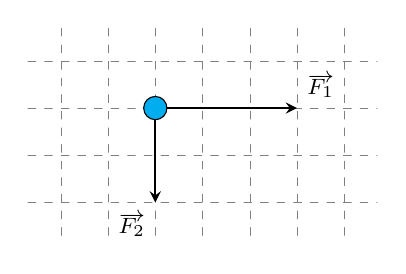
\begin{tikzpicture}[>=stealth,scale=0.6, line join=round, line cap=round]
			\draw[line width=0.05pt,gray,dashed] (-2.7,-0.7) grid (4.7,3.7);
			\draw[->,thick](0,2)--(0,0)node[below left]{\footnotesize$\overrightarrow{F_2}$};
			\draw[->,thick](0,2)--(3,2)node[above right]{\footnotesize$\overrightarrow{F_1}$};
			\draw[fill=cyan] (0,2) circle(7pt);
	\end{tikzpicture}}
\end{vd}

\begin{vd}
	\immini
	{
		Cho hai lực $\overrightarrow{F}_{1}=\overrightarrow{M A}$,  $\overrightarrow{F}_{2}=\overrightarrow{M B}$ cùng tác động vào một vật tại điểm $M$ cường độ hai lực $\overrightarrow{F}_{1}$, $\overrightarrow{F}_{2}$ đều bằng $300$ (N) và $\widehat{AMB}=60^{\circ}$. Tìm cường độ của lực tổng hợp tác động vào vật.
	}
	{	\begin{tikzpicture}[smooth,font=\footnotesize,scale=0.8, >=Latex]
			\path
			(0,0) coordinate (M)
			(3,0) coordinate (A)
			($(M)!1!60:(A)$)coordinate (B);
			\fill[ball color=red](M) circle (0.16);
			\draw[->] (M)--(A);
			\draw[->] (M)--(B);
			\foreach \x/\g in {A/0,B/60,M/-90} \draw [fill=black] (\x) circle (.05) + (\g:.5) node{$\x$};
			\begin{scope}
				\clip (B)--(M)--(A);
				\draw[double] (M) circle(0.7cm);
			\end{scope}
		\node[right] at (0.6,0.5) {$60^\circ$};
	\end{tikzpicture}
}
	\loigiai{
		\immini
		{
			Gọi $D$ là đỉnh thứ tư của hình thoi $MBDA$, ta có 
			$$\overrightarrow{MA}+\overrightarrow{MB}=\overrightarrow{MD}.$$
			Vậy cường độ lực tổng hợp tại $M$ là 
			$\left|\overrightarrow{MD}\right|=MD$.
		}
		{
			\begin{tikzpicture}[smooth,font=\footnotesize,scale=0.8, >=Latex]
				\path
				(0,0) coordinate (M)
				(3,0) coordinate (A)
				($(M)!1!60:(A)$)coordinate (B)
				($(A)+(B)-(M)$)coordinate (D);
				\fill[ball color=red](M) circle (0.16);
				\draw[->] (M)--(A);
				\draw[->] (M)--(B);
				\draw[->] (M)--(D);
				\draw[dashed] (B)--(D)--(A);
				\foreach \x/\g in {A/0,B/60,M/-90,D/0} \draw [fill=black] (\x) circle (.05) + (\g:.5) node{$\x$};
				\begin{scope}
					\clip (B)--(M)--(A);
					\draw[double] (M) circle(0.7cm);
				\end{scope}
				\node[right] at (0.6,0.35) {\tiny$60^\circ$};
			\end{tikzpicture}	
		}
		\noindent 
		Gọi $O$ là tâm hình thoi $MBDA$ có cạnh $300$, ta có 
		$MD=2MO=300 \sqrt 3$ (N).
	}
\end{vd}

\begin{vd}
	\immini{Tính lực kéo cần thiết để kéo một khẩu pháo có trọng lượng 22 148 N (xấp xỉ 2 260 kg) lên một con dốc nghiêng $30^\circ$ so với phương nằm ngang (hình bên). Nếu lực kéo của mỗi người bằng 100 N thì cần tối thiểu bao nhiêu người để kéo pháo (\textit{bỏ qua ma sát trượt giữa bánh xe và mặt phẳng nghiêng})?}{
	\begin{tikzpicture}[thick, font=\small, >=Latex]
		\draw (0,0)coordinate(O)
		($(O)+(0:4.5)$)coordinate(O1)
		($(O)+(30:4.55)$)coordinate(O2)
		($(O)+(30:2.8)$)coordinate(O3)
		($(O3)!0.32 cm!90:(O2)$)coordinate(A1)
		;
		\draw[cyan] (O1)--(O)--(O2)
		($(O)!0.5 cm!(O1)$) to [bend right=40]node[shift={(15:0.4)}]{\scriptsize$30^\circ$} ($(O)!0.5 cm!(O2)$)
		;
		%% -- Thân pháo
		\path 
		($(A1)+(120:0.4)$)coordinate(B1)
		($(B1)+(30:0.4)$)coordinate(B2)
		($(B1)+(210:0.5)$)coordinate(B3)
		($(B3)+(-60:0.1)$)coordinate(B4)
		($(B1)+(210:0.1)+(-60:0.02)$)coordinate(C1)
		($(C1)+(120:0.25)$)coordinate(B5)
		($(B5)+(28:1)$)coordinate(B6)
		($(C1)+(32:1)$)coordinate(B7)
		;
		%% fill pháo
		\shade [top color=darkgray, bottom color = black, middle color =lightgray, shading angle=30] (C1)..controls++(210:0.2)and++(210:0.2)..(B5)--(B6)..controls++(28:0.02)and++(32:0.01)..(B7)--(C1) ;
		%\fill bệ pháo
		\fill [darkgray] (A1) ..controls++(220:0.3) and++(30:0.5)..(B4)..controls++(210:0.1)and++(210:0.1)..(B3)--(B2)..controls++(30:0.2)and++(40:0.1)..(A1)
		;
		%%- Bánh xe
		\fill [white] (A1) circle (0.3 cm) ; 
		\foreach \a in {0,30,...,360}{
			\draw [line width=1pt, blue] (A1)--++(\a:0.3);
		}
		\draw [blue, line width=1.5pt] (A1) circle (0.3 cm);
		\fill [black] (A1) circle (0.05 cm);
		%% -- Vẽ Vecto
		\draw [dashed] ($(A1)+(-90:1.5)$)coordinate(DA)node[right]{$A$}
		(A1)++(210:0.5)coordinate(C1)
		(DA)++(120:1)coordinate(DA1)
		(intersection = of DA--DA1 and A1--C1)coordinate(DC)node[left]{$C$}
		(A1)++(120:1)coordinate(DB1)
		(DC)++(90:1)coordinate(DC1)
		(intersection = of DC--DC1 and A1--DB1)coordinate(DB)node[above left]{$B$}
		(DA)--(DC)--(DB)
		(A1)node[below right=5pt]{$O$}
		;
		\draw [->] (A1) --(DA) ;
		\draw [->] (A1) --(DB) ;
		\draw [->, dashed] (A1) --(DC) ;
		\draw [->] (A1) --++(30:1.5)node[above]{$\overrightarrow{F}$} ; %% Độ dài vecto F
\end{tikzpicture}}
\loigiai{
	\immini{
	Lực tổng hợp của trọng lực $\vec{P}$ và phản lực $\vec{w}$ là lực $\vec{T}=\vec{OC}$. Theo hình vẽ thì
	$$\big|\vec{T}\big|=OC=OA \cdot \sin 30^\circ=11074\, \mathrm{N}$$
	Suy ra, muốn kéo được pháo lên dốc thì lực $\vec{F}$ phải có độ lớn
	$$\big|\vec{F}\big|>\big|\vec{T}\big|=11074\, \mathrm{N}$$
	Do $\dfrac{11074}{100}=110,74$ nên nếu lực kéo mỗi người là 100 N thì ta cần tối thiểu 111 người.}{
	
	\begin{tikzpicture}[smooth,font=\footnotesize,scale=0.8,>= Latex]
		\path
		(0,0) coordinate (M)
		(7,0) coordinate (N)
		($(M)!1!30:(N)$) coordinate (P)
		%Dữ liệu vật trên mặt phẳng nghiên 30 độ
		($(M)!0.5!(P)$) coordinate (X)
		($(M)!0.7!(P)$) coordinate (X')
		($(X)!0.3!90:(X')$) coordinate (Y)
		($(X')!0.3!-90:(X)$) coordinate (Y')
		% Dữ liệu lực F
		($(X')!0.5!(Y)$) coordinate (O)
		($(X')!0.5!(Y')$) coordinate (I)
		($(O)!3!(I)$) coordinate (F)
		%Dữ liệu trọng lực
		($(O)!2.5!-120:(I)$) coordinate (A)
		% Dữ liệu vecto phân tích trọng lực P và phàn lực w
		($(M)!(A)!(P)$) coordinate (A')
		(intersection of A--A' and O--F) coordinate (C)
		% Dữ liệu phản lực
		($(O)+(C)-(A)$) coordinate (B)
		;
		\draw (N)--(M)--(P);
		\fill[cyan] (X)--(Y)--(Y')--(X');
		\draw[->] (O)--(F)node[above]{$\vec{F}$};
		\draw[->] (O)--(A)node[shift={(70:0.7)}]{\scriptsize$\vec{P}$};
		\draw[->] (O)--(B)node[shift={(-30:0.6)}]{\scriptsize$\vec{w}$};
		\draw[->,dashed] (O)--(C);
		\draw[dashed] (A)--(C)--(B);
		\foreach \x/\g in {O/-20,A/0,B/80,C/180} \draw [fill=black] (\x) circle (.05) + (\g:.3) node{$\x$};
		\begin{scope}
			\clip (N)--(M)--(P);
			\draw[double] (M) circle(0.6cm);
		\end{scope}
		\begin{scope}
			\clip (O)--(A)--(C);
			\draw[double] (A) circle(0.6cm);
		\end{scope}
		\node[right] at (0.6,0.25) {\scriptsize$30^\circ$};
		\node[right] at (3,1.32) {\tiny$30^\circ$};
\end{tikzpicture}}}
\end{vd}

\begin{vd}
	\immini{Hai con tàu xuất phát cùng lúc từ bờ bên này để sang bờ bên kia của dòng sông (hai bờ song song nhau) với vận tốc riêng không đổi và có độ lớn bằng nhau. Hai tàu luôn giữ lái sao cho chúng tạo với bờ cùng một góc nhọn nhưng một tàu hướng xuống hạ lưu, một tàu hướng lên thượng nguồn. Vận tốc dòng nước là đáng kể, các yếu tố bên ngoài khác không ảnh hưởng tới vận tốc của các tàu. Hỏi tàu nào sang bờ bên kia trước?}{
		\begin{tikzpicture}[scale=0.7]
			\def\dai{6}
			\def\rong{4}
			\draw (0,0)coordinate(SW) --++(0:\dai)coordinate(SE)
			(SW)++(90:\rong)coordinate(NW)
			(SE)++(90:\rong)coordinate(NE)
			
			;
			%% Màu nước
			\fill [cyan!70!white] (NW) rectangle (SE); 
			%% màu đất
			\fill [brown] (NW) rectangle ($(NE)!0.05!(SE)$) (SW) rectangle ($(SE)!0.15!(NE)$) ;
			%% màu cỏ 
			\fill [green!70!blue] (SW) rectangle ($(SE)!0.1!(NE)$)
			;
			\draw ($(SW)!0.15!(NW)+(0.35*\dai,0)$)coordinate(A)
			($(SW)!0.15!(NW)+(0.55*\dai,0)$)coordinate(B)
			($(A)+(120:1.3)$)coordinate(A1)
			($(B)+(60:1.3)$)coordinate(B1)
			($(A)!0.55!(A1)$)coordinate(A2)
			($(B)!0.55!(B1)$)coordinate(B2)
			($(A)!0.25!(A1)$)coordinate(A3)
			($(B)!0.25!(B1)$)coordinate(B3)
			;
			\tikzset{song/.pic={
					\draw [white] (0,0)..controls++(150:0.6)and++(-50:0.3)..++(-0.1,0.5)..controls++(150:0.2)and++(200:0.1)..++(0.0,0.3)
					; }}
			\foreach \a/\b in {-0.8/2,-1/1,-1.1/2.5}{
				\draw [opacity=0.6] ($(SE)+(\a,\b)$)pic{song}
				;}
			
			%% Vẽ thuyền bên phải, màu đỏ
			\shadedraw [top color = red!80!white, bottom color=red, draw=black!30!blue] (B)..controls++(20:0.4)and++(-80:0.4)..(B1)..controls++(-160:0.4)and++(100:0.4)..(B);
			%% Vẽ thuyền bên trái màu cam
			\shadedraw [top color = orange!80!white, bottom color=orange, draw=black!30!red] (A)..controls++(80:0.4)and++(-20:0.4)..(A1)..controls++(-100:0.4)and++(160:0.4)..(A) ;
			%% Vẽ khoang ngồi thuyền phải 
			\shade [ top color = red!60!black, bottom color = red!80!black,  rounded corners=0.05cm] (B2)--++(-30:0.11)--++(60:0.3)--++(150:0.22)--++(240:0.3)--cycle
			(B3)--++(-30:0.11)--++(60:0.3)--++(150:0.22)--++(240:0.3)--cycle;
			%% Vẽ khoang ngồi thuyền trái
			\shade [ top color = orange!60!black, bottom color = orange!80!black,  rounded corners=0.05cm] (A2)--++(30:0.11)--++(120:0.3)--++(210:0.22)--++(-60:0.3)--cycle
			(A3)--++(30:0.11)--++(120:0.3)--++(210:0.22)--++(-60:0.3)--cycle;
			%% Vẽ nón lá người ngồi chèo
			\shade [top color = yellow!50!yellow!40!white, bottom color =yellow!50!yellow!50!white, shading angle=30 , draw =black, line width=0.1pt] (B3) circle (0.17 cm) 
			(A3) circle (0.17 cm) ;
			\foreach \a in {0,15,...,360}{
				\draw [line width=0.1pt , black] (B3)--++(\a:0.17) (A3)--++(\a:0.17) ;
			}
			%% Fill điểm đen
			\fill [black] (A) circle (2pt) (B) circle (2pt) ;
			%% Mũi tên định hướng thuyền
			\draw [->, >=Latex, black , line width=0.5pt] (A1)--++(120:0.5) ; % thuyền cam
			\draw [->, >=Latex, black, line width=0.5pt] (B1)--++(60:0.5) ; % thuyền đỏ
			
		\end{tikzpicture}
	}
\loigiai{
}
\end{vd}
\baitaptl
%%==========Câu 1
\begin{bt}
	\immini
	{
		Cho hai lực $\overrightarrow{F}_{1}=\overrightarrow{M A}$,  $\overrightarrow{F}_{2}=\overrightarrow{M B}$ cùng tác động vào một vật tại điểm $M$ cường độ hai lực $\overrightarrow{F}_{1}$, $\overrightarrow{F}_{2}$ lần lượt là $300$ (N) và $400$ (N) và $\widehat{AMB}=90^{\circ}$. Tìm cường độ của lực tổng hợp tác động vào vật.
	% 	\choice
	% 	{$0$ (N)}
	% 	{$700$ (N)}
	% 	{$100$ (N)}
	% 	{\True $500$ (N)}	
	}
	{
		\begin{tikzpicture}[>=stealth,line join=round,line cap=round,font=\footnotesize,scale=0.8]
			\path (0,0) coordinate (M)
			(3,0) coordinate (A)
			(0,4) coordinate (B)
			;
			\draw[->] (M)--(A);
			\draw[->] (M)--(B);
			
			\foreach \p/\r in {A/90,M/180,B/0}
			\draw (\p)  node[shift={(\r:3mm)}]{$\p$};
	\end{tikzpicture}	}
	\loigiai{
		\immini
		{
			Gọi $D$ là đỉnh thứ tư của hình chữ nhật $MADB$, ta có 
			$$\overrightarrow{MA}+\overrightarrow{MB}=\overrightarrow{MD}.$$
			Vậy cường độ lực tổng hợp tại $M$ là 
			$\left|\overrightarrow{MD}\right|=MD=\sqrt{MB^2+MA^2}=500$ (N).
		}
		{
			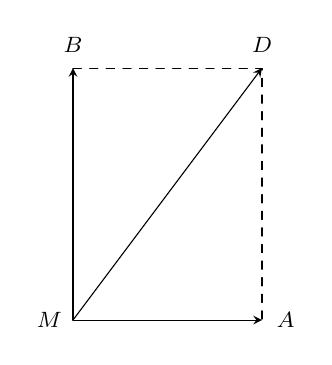
\begin{tikzpicture}[>=stealth,line join=round,line cap=round,font=\footnotesize,scale=0.8]
				\path (0,0) coordinate (M)
				(3,0) coordinate (A)
				(0,4) coordinate (B)
				(3,4) coordinate (D)
				;
				\draw[->] (M)--(A);
				\draw[->] (M)--(B);
				\draw[->] (M)--(D);
				\draw[dashed] (B)--(D)--(A);
				
				\foreach \p/\r in {A/0,M/180,B/90,D/90}
				\draw (\p)  node[shift={(\r:3mm)}]{$\p$};
			\end{tikzpicture}	
		}
	}
\end{bt}
% \baitaptl 

%%==========Câu 2
\begin{bt}
	\immini
	{
		Cho hai lực $\overrightarrow{F}_{1}=\overrightarrow{M A}$,  $\overrightarrow{F}_{2}=\overrightarrow{M B}$ cùng tác động vào một vật tại điểm $M$ cường độ hai lực $\overrightarrow{F}_{1}$, $\overrightarrow{F}_{2}$ đều bằng $300$ (N) và $\widehat{AMB}=60^{\circ}$. Tìm cường độ của lực tổng hợp tác động vào vật.
		% \choice
		% {$0$ (N)}
		% {$300$ (N)}
		% {\True $300\sqrt 3$ (N)}
		% {$500$ (N)}	
	}
	{
		\begin{tikzpicture}[>=stealth,line join=round,line cap=round,font=\footnotesize,scale=0.8]
			\path (0,0) coordinate (M)
			(3,0) coordinate (A)
			(60:3) coordinate (B)
			;
			\draw[->] (M)--(A);
			\draw[->] (M)--(B);
			% \tkzMarkAngles[size=1,arc=ll,mark={}](A,M,B)
			\draw (M) node[above right]{$60^\circ$};
			\foreach \p/\r in {A/90,M/180,B/0}
			\draw (\p)  node[shift={(\r:3mm)}]{$\p$};
	\end{tikzpicture}	}
	\loigiai{
		\immini
		{
			Gọi $D$ là đỉnh thứ tư của hình thoi $MBDA$, ta có 
			$$\overrightarrow{MA}+\overrightarrow{MB}=\overrightarrow{MD}.$$
			Vậy cường độ lực tổng hợp tại $M$ là 
			$\left|\overrightarrow{MD}\right|=MD$.
		}
		{
			\begin{tikzpicture}[>=stealth,line join=round,line cap=round,font=\footnotesize,scale=0.8]
				\path (0,0) coordinate (M)
				(2,0) coordinate (A)
				(60:2) coordinate (B)
				(30:3.464101615) coordinate (D)
				($(B)!1/2!(A)$) coordinate (O)
				;
				\draw[->] (M)--(A);
				\draw[->] (M)--(B);
				\draw[->] (M)--(D);
				\draw[dashed] (B)--(D)--(A) (B)--(A);
				% \tkzMarkAngles[size=1cm,arc=ll,mark={}](A,M,B)
				% \draw (M) node[above=0.2, rotate=20]{$60^\circ$};
				\foreach \p/\r in {A/0,M/180,B/90,D/90,O/60}
				\draw (\p)  node[shift={(\r:3mm)}]{$\p$};
			\end{tikzpicture}	
		}
		\noindent 
		Gọi $O$ là tâm hình thoi $MBDA$ có cạnh $300$, ta có 
		$MD=2MO=300 \sqrt 3$ (N).
	}
\end{bt}


\subsection{Câu hỏi trắc nghiệm}
\Opensolutionfile{ansbook}[ans/ansbook-2D1-2-TN]
\Opensolutionfile{ans}[ans/ans-0H1-8-TN]
\begin{ex}%[BG1-2022-Huỳnh Xuân Tín]%[0H1Y2-2]
	Cho ba điểm phân biệt $A$, $B$, $C$. Đẳng thức nào sau đây đúng?
	\choice
	{\True $\overrightarrow{CA} - \overrightarrow{BA} = \overrightarrow{CB}$}
	{$\overrightarrow{AB} + \overrightarrow{AC} = \overrightarrow{CB}$}
	{$\overrightarrow{AB} + \overrightarrow{CA} = \overrightarrow{BC}$}
	{$\overrightarrow{AB} - \overrightarrow{AC} = \overrightarrow{BC}$}
	\loigiai{
		Ta có $\overrightarrow{CA} - \overrightarrow{BA} = \overrightarrow{CA} + \overrightarrow{AB} = \overrightarrow{CB}$. \\
		Mặt khác
		\begin{itemize}
			\item $\overrightarrow{AB} + \overrightarrow{AC} = \overrightarrow{AC} + \overrightarrow{CB} + \overrightarrow{AC} = 2\overrightarrow{AC} + \overrightarrow{CB} \ne \overrightarrow{CB}$. 
			\item $\overrightarrow{AB} + \overrightarrow{CA} = \overrightarrow{CA} + \overrightarrow{AB} = \overrightarrow{CB} \ne \overrightarrow{BC}$.
			\item $\overrightarrow{AB} - \overrightarrow{AC} = \overrightarrow{CB} \ne \overrightarrow{BC}$.
		\end{itemize}	
	}
\end{ex}

\begin{ex}%[BG1-2022-Huỳnh Xuân Tín]%[0H1B2-4]
	Rút gọn biểu thức vectơ $\vec{AM}+\vec{MB}-\vec{AC}$ ta được kết quả đúng là
	\choice
	{$\vec{MB}$}
	{$\vec{BC}$}
	{\True $\vec{CB}$}
	{$\vec{AB}$}
	\loigiai{
		Ta có $\vec{AM}+\vec{MB}-\vec{AC}=\vec{AB}-\vec{AC}=\vec{CB}$.
	}
\end{ex}
\begin{ex}%[BG1-2022-Huỳnh Xuân Tín]%[0H1B2-4]
	Gọi $O$ là tâm hình vuông $ABCD$. Tính $\overrightarrow{OB}-\overrightarrow{OC}$.
	\choice
	{$\overrightarrow{OB}-\overrightarrow{OC}=\overrightarrow{BC}$}
	{\True $\overrightarrow{OB}-\overrightarrow{OC}=\overrightarrow{DA}$}
	{$\overrightarrow{OB}-\overrightarrow{OC}=\overrightarrow{OD}-\overrightarrow{OA}$}
	{$\overrightarrow{OB}-\overrightarrow{OC}=\overrightarrow{AB}$}
	\loigiai{
		Ta có $\overrightarrow{OB}-\overrightarrow{OC}=\overrightarrow{CB}=\overrightarrow{DA}$. }
\end{ex}


\begin{ex}%[BG1-2022-Huỳnh Xuân Tín]%[0H1B2-1]
	Cho bốn điểm $A$, $B$, $C$, $D$ phân biệt và $\vec{u}=\vec{AD}+\vec{CD}-\vec{CB}-\vec{BD}$. Khẳng định nào sau đây đúng?
	\choice
	{$\vec{u}=\vec{0}$}
	{\True $\vec{u}=\vec{AD}$}
	{$\vec{u}=\vec{CD}$}
	{$\vec{u}=\vec{AC}$}
	\loigiai{
		Ta có $\vec{u}=\vec{AD}+\vec{CD}-\vec{CB}-\vec{BD}=\vec{AD}+\vec{BD}-\vec{BD}=\vec{AD}$.
	}
\end{ex}
\begin{ex}%[BG1-2022-Huỳnh Xuân Tín]%[0H1B2-1]
	\immini
	{
		Cho hình bình hành $ABCD$ tâm $O$ . Hỏi vectơ $\overrightarrow{AO}-\overrightarrow{DO}$ bằng vectơ nào trong các vectơ sau?
		\choicew{0.25\textwidth}
		\choice
		{$\overrightarrow{BA}$}
		{\True $\overrightarrow{BC}$}
		{$\overrightarrow{DC}$}
		{$\overrightarrow{AC}$}	
	}
	{
		\begin{tikzpicture}[scale=0.9, font=\footnotesize, line join = round, line cap = round,>=stealth]
			\tkzDefPoints{0/0/A,1/1.5/B,3/0/D}
			\coordinate (C) at ($(B)+(D)-(A)$);
			\tkzDefMidPoint(A,C) \tkzGetPoint{O}
			\tkzDrawPoints[fill=black](A,B,C,D,O)
			\tkzDrawPolygon(A,B,D,C)
			\tkzDrawSegments(C,B A,D)
			\tkzLabelPoints[above](B,C)
			\tkzLabelPoints[below](A,D,O) 
		\end{tikzpicture}	
	}	
	\loigiai{
		Ta có $\overrightarrow{AO}-\overrightarrow{DO}=-\overrightarrow{OA}+\overrightarrow{OD}=\overrightarrow{OD}-\overrightarrow{OA}=\overrightarrow{AD}=\overrightarrow{BC}$. }
\end{ex}

\begin{ex}%[BG1-2022-Huỳnh Xuân Tín]%[0H1B2-1]
	Cho tam giác $ABC$. Gọi $M, N, P$ lần lượt là trung điểm các cạnh $AB$, $AC$, $BC$. Tổng $\vec{MP}+\vec{NP}$ bằng vectơ nào?
	\choice
	{$\vec{PA}$}
	{$\vec{AM}$}
	{$\vec{PB}$}
	{\True $\vec{AP}$}
	\loigiai
	{ \immini[thm]{Ta có tứ giác $MANP$ là hình bình hành.\\
			Mà $\vec{MP}+\vec{NP}=-\left( \vec{PM}+\vec{PN}\right) =- \vec{PA} =\vec{AP}.$
		}
		{\begin{tikzpicture}[scale=0.6, line join=round, line cap=round]
				\clip (-1.5,-1.5) rectangle (4.5,3.5);
				\tkzDefPoints{-1/0/B,1/3/A,4/0/C}
				\coordinate (M) at ($(A)!0.5!(B)$);
				\coordinate (N) at ($(A)!0.5!(C)$);
				\coordinate (P) at ($(C)!0.5!(B)$);
				
				\tkzDrawPoints[size=5,fill=black](A,B,C,M,N,P)
				\tkzLabelPoints[left](M)
				\tkzLabelPoints[right](N)
				\tkzLabelPoints[below](B,C,P)
				\tkzLabelPoints[above](A)
				\tkzDrawPolygon(A,B,C)
				\tkzDrawPolygon(M,N,P)
				\tkzDrawSegments(P,A)
				
		\end{tikzpicture}}
	}
\end{ex}
\begin{ex}%[BG1-2022-Huỳnh Xuân Tín]%[0H1B2-2]
	\immini
	{
		Cho lục giác đều $ABCDEF$ có tâm $O$. Đẳng thức nào sau đây \textbf{sai}? 
		\choicew{0.5\textwidth}
		\choice
		{$\overrightarrow{OA}+\overrightarrow{OC}+\overrightarrow{OE}=\overrightarrow{0}$}
		{$\overrightarrow{OA}+\overrightarrow{OC}+\overrightarrow{OB}=\overrightarrow{EB}$}
		{$\overrightarrow{AB}+\overrightarrow{CD}+\overrightarrow{EF}=\overrightarrow{0}$}
		{\True $\overrightarrow{BC}+\overrightarrow{EF}=\overrightarrow{AD}$}	
	}
	{
		\begin{tikzpicture}[scale=0.7, font=\footnotesize, line join = round, line cap = round,>=stealth]
			\tkzDefPoints{0/0/O,2/0/A}
			\tkzDefPointBy[rotation = center O angle 60](A)    \tkzGetPoint{B}
			\tkzDefPointBy[rotation = center O angle 60](B)    \tkzGetPoint{C}
			\tkzDefPointBy[rotation = center O angle 60](C)    \tkzGetPoint{D}
			\tkzDefPointBy[rotation = center O angle 60](D)    \tkzGetPoint{E}
			\tkzDefPointBy[rotation = center O angle 60](E)    \tkzGetPoint{F}
			\tkzDrawPoints[fill=black](A,B,C,D,E,F,O)
			\tkzDrawPolygon(A,B,C,D,E,F)
			\tkzDrawSegments(A,D B,E C,F)
			\tkzLabelPoints[above](B,C)  
			\tkzLabelPoints[below](E,F,O)
			\tkzLabelPoints[left](D)  
			\tkzLabelPoints[right](A)	
		\end{tikzpicture}	
	}
	\loigiai{
		Ta có \\
		$\overrightarrow{OA}+\overrightarrow{OC}+\overrightarrow{OE}=\left(\overrightarrow{OA}+\overrightarrow{OC}\right)+\overrightarrow{OE}=\overrightarrow{OB}+\overrightarrow{OE}=\overrightarrow{0}$  đúng.\\
		$\overrightarrow{OA}+\overrightarrow{OC}+\overrightarrow{OB}=\left(\overrightarrow{OA}+\overrightarrow{OC}\right)+\overrightarrow{OB}$
		$=\overrightarrow{OB}+\overrightarrow{OB}=2\overrightarrow{OB}=\overrightarrow{EB}$ đúng.\\
		$\overrightarrow{AB}+\overrightarrow{CD}+\overrightarrow{EF}=\left(\overrightarrow{AB}+\overrightarrow{BO}\right)+\overrightarrow{OA}=\overrightarrow{AO}+\overrightarrow{OA}=\overrightarrow{AA}=\overrightarrow{0}$  đúng.}
\end{ex}



\begin{ex}%[BG1-2022-Huỳnh Xuân Tín]%[0H1B2-4]
	Cho hình bình hành $ABCD$. vectơ $\vec{BC}-\vec{AB}$ bằng vectơ nào dưới đây?
	\choice
	{$\vec{DB}$}
	{$\True \vec{BD}$}
	{$\vec{AC}$}
	{$\vec{CA}$}
	\loigiai{$\vec{BC}-\vec{AB}=\vec{BC}+\vec{BA}=\vec{BD}$.}
\end{ex}
\begin{ex}%[BG1-2022-Huỳnh Xuân Tín]%[0H1B2-4]
	\immini
	{
		Cho hình bình hành $ABCD$. Gọi $G$ là trọng tâm của tam giác $ABC$. Mệnh đề nào sau đây đúng?
		\choice
		{\True $\overrightarrow{GA}+\overrightarrow{GC}+\overrightarrow{GD}=\overrightarrow{BD}$}
		{$\overrightarrow{GA}+\overrightarrow{GC}+\overrightarrow{GD}=\overrightarrow{CD}$}
		{$\overrightarrow{GA}+\overrightarrow{GC}+\overrightarrow{GD}=\overrightarrow{O}$}
		{$\overrightarrow{GA}+\overrightarrow{GD}+\overrightarrow{GC}=\overrightarrow{CD}$}	
	}
	{
		\begin{tikzpicture}[scale=0.9, font=\footnotesize, line join = round, line cap = round,>=stealth]
			\tkzDefPoints{0/0/D,2/2/A,4/0/C}
			\coordinate (B) at ($(A)+(C)-(D)$);
			\tkzCentroid(A,B,C)    \tkzGetPoint{G}
			\tkzDrawPoints[fill=black](A,B,C,D,G)
			\tkzDrawPolygon(A,B,D,C)
			\tkzDrawSegments(C,B A,D G,A G,C)
			\tkzLabelPoints[above](B,A,G)
			\tkzLabelPoints[below](C,D) 
		\end{tikzpicture}		
	}	
	\loigiai{
		Vì $G$ là trọng tâm của tam giác $ABC$ nên 
		$\overrightarrow{GA}+\overrightarrow{GB}+\overrightarrow{GC}=\overrightarrow{0}\Rightarrow \overrightarrow{GA}+\overrightarrow{GC}=-\overrightarrow{GB}$.\\
		Do đó $\overrightarrow{GA}+\overrightarrow{GC}+\overrightarrow{GD}=-\overrightarrow{GB}+\overrightarrow{GD}=\overrightarrow{GD}-\overrightarrow{GB}=\overrightarrow{BD}$. 
	}
\end{ex}


\begin{ex}%[BG1-2022-Huỳnh Xuân Tín]%[0H1Y2-2]
	Chọn mệnh đề \textbf{sai} trong các mệnh đề sau.
	\choice
	{\True Nếu $\vec{a}+\vec{b}=\vec{c}$ thì $\left| \vec{a}\right|+\left| \vec{b}\right|=\left| \vec{c}\right|$}
	{$\vec{FY}-\vec{BY}=\vec{FB}$ với $B$, $F$, $Y$ bất kì}
	{Nếu $ABCD$ là hình bình hành thì $\vec{AB}+\vec{AD}=\vec{AC}$}
	{$\vec{AM}+\vec{MH}=\vec{AH}$  với $A$, $M$, $H$ bất kì}
	\loigiai{
		Mệnh đề sai: Nếu $\vec{a}+\vec{b}=\vec{c}$ thì $\left| \vec{a}\right|+\left| \vec{b}\right|=\left| \vec{c}\right|$.		
	}
\end{ex}
%2
% \begin{ex}%[BG1-2022-Huỳnh Xuân Tín]%[0H1Y2-2]
% 	Cho ba điểm phân biệt $A,B,C$. Đẳng thức nào sau đây là \textbf{đúng} ?
% 	\choice
% 	{ $\vec{AB}+\vec{AC}=\vec{BC}$}
% 	{$\vec{CA}-\vec{BA}=\vec{BC} $}
% 	{\True $ \vec{AB}+\vec{CA}=\vec{CB}$}
% 	{$ \vec{AB}-\vec{BC}=\vec{CA}$}
% 	\loigiai{Áp dụng quy tắc ba điểm $ \vec{CA}+\vec{AB}=\vec{CB}$.
		
% 	}
% \end{ex}
% %3
% \begin{ex}%[BG1-2022-Huỳnh Xuân Tín]%[0H1Y2-1]
% 	Rút gọn biểu thức  $\overrightarrow{AM}+\overrightarrow{MB}-\overrightarrow{AC}$ ta được kết quả nào dưới đây?
% 	\choice
% 	{$\overrightarrow{MB}$}
% 	{$\overrightarrow{BC}$}
% 	{\True $\overrightarrow{CB}$}
% 	{$\overrightarrow{AB}$}
% 	\loigiai
% 	{Ta có $\overrightarrow{AM}+\overrightarrow{MB}-\overrightarrow{AC} = \overrightarrow{AB} - \overrightarrow{AC} = \overrightarrow{CB}$.
% 	}
% \end{ex}


\begin{ex}%[BG1-2022-Huỳnh Xuân Tín]%[0H1B2-2]
	Trong mặt phẳng cho bốn điểm bất kì $A,B,C,O$. Đẳng thức nào sau đây là đúng?
	\choice
	{$\overrightarrow{AB}=\overrightarrow{OB}+\overrightarrow{OA}$}
	{$\overrightarrow{AB}=\overrightarrow{AC}+\overrightarrow{BC}$}
	{\True $\overrightarrow{OA}=\overrightarrow{CA}-\overrightarrow{CO}$}
	{$\overrightarrow{OA}=\overrightarrow{OB}-\overrightarrow{BA}$}
	\loigiai{
		Nhắc lại lý thuyết: Với $3$ điểm $O,A,B$ bất kì:\\
		Quy tắc $3$ điểm: $\overrightarrow{OA}+\overrightarrow{AB}=\overrightarrow{OB}$.\\
		Quy tắc hiệu: $\overrightarrow{OA}-\overrightarrow{OB}=\overrightarrow{BA}$.
	}
\end{ex}
%8
\begin{ex}%[BG1-2022-Huỳnh Xuân Tín]%[0H1B2-2]
	Cho ba điểm $A,B,C$ phân biệt. Đẳng thức nào sau đây là \textbf{sai}?
	\choice
	{\True $\overrightarrow{AC}+\overrightarrow{AB}=\overrightarrow{CB}$}
	{$\overrightarrow{AB}+\overrightarrow{BC}=\overrightarrow{AC}$}
	{$\overrightarrow{AC}-\overrightarrow{AB}=\overrightarrow{BC}$}
	{$\overrightarrow{AC}-\overrightarrow{BC}=\overrightarrow{AB}$}
	\loigiai{
		Nhắc lại lý thuyết: Với $3$ điểm $C,A,B$ bất kì:\\
		Quy tắc $3$ điểm: $\overrightarrow{CA}+\overrightarrow{AB}=\overrightarrow{CB}$.\\
		Quy tắc hiệu: $\overrightarrow{CA}-\overrightarrow{CB}=\overrightarrow{BA}$.
	}
\end{ex}

%9
\begin{ex}%[BG1-2022-Huỳnh Xuân Tín]%[0H1K2-1]
	Tổng $\overrightarrow{MN}+\overrightarrow{PQ}+\overrightarrow{RN}+\overrightarrow{NP}+\overrightarrow{QR}$ bằng
	\choice
	{$\overrightarrow{MR}$}
	{\True $\overrightarrow{MN}$}
	{$\overrightarrow{MP}$}
	{$\overrightarrow{MQ}$}
	\loigiai{Ta có $\overrightarrow{MN}+\overrightarrow{PQ}+\overrightarrow{RN}+\overrightarrow{NP}+\overrightarrow{QR}=\overrightarrow{MN}+\overrightarrow{NP}+\overrightarrow{PQ}+\overrightarrow{QR}+\overrightarrow{RN}=\overrightarrow{MN}$.}
\end{ex}
%10

\begin{ex}%[BG1-2022-Huỳnh Xuân Tín]%[0H1K2-2]
	Cho $4$ điểm bất kì $A,B,C,D$. Đẳng thức nào sau đây sai?
	\choice
	{$\overrightarrow{AB}=\overrightarrow{AC}+\overrightarrow{BC}$}
	{\True $\overrightarrow{DA}=\overrightarrow{BD}-\overrightarrow{CD}$}
	{$\overrightarrow{AB}=\overrightarrow{DB}-\overrightarrow{DA}$}
	{$\overrightarrow{BC}=\overrightarrow{BD}+\overrightarrow{DC}$}
	\loigiai{Ta có $\overrightarrow{BD}-\overrightarrow{CD}=\overrightarrow{BC}$.}
\end{ex}


\begin{ex}%[BG1-2022-Huỳnh Xuân Tín]%[0H1B2-1]
	Cho bốn điểm $A, B, C$. Tính  $\vec{AB}-\vec{AC}$.
	\choice
	{$\vec{CA}$}
	{$2\cdot \vec{AC}$}
	{$\vec{0}$}
	{\True $\vec{AC}$}
	\loigiai{
		$\vec{AB}-\vec{AC}=\vec{AC}$.		
	}
\end{ex}

%2

\begin{ex}%[BG1-2022-Huỳnh Xuân Tín]%[0H1B2-2]
	Cho tam giác $ABC$ và điểm $M$ bất kỳ, chọn đẳng thức \textbf{đúng}.
	\choice
	{$\vec{AB}-\vec{AC}=\vec{BC}$}
	{$\vec{MA}+\vec{BM}=\vec{AB}$}
	{\True $\vec{MB}-\vec{MC}=\vec{CB}$}
	{$\vec{AA}-\vec{BB}=\vec{AB}$}
	\loigiai{Áp dụng quy tắc công, trừ.
		Ta có: $\vec{AB}-\vec{AC}=\vec{CA}$\\
		$\vec{MA}+\vec{BM}=\vec{BM}+\vec{MA}=\vec{BA}$\\
		$\vec{AA}-\vec{BB}=\vec{0}$
}\end{ex}

\begin{ex}%[BG1-2022-Huỳnh Xuân Tín]%[0H1B2-1]
	Cho hình bình hành $ABCD$. Gọi $M$, $N$ lần lượt là trung điểm $BC$ và $AD$. Tổng của $\vec{NC}$ và $\vec{MC}$ là 
	\choice
	{$\vec{0}$}
	{$\vec{MN}$}
	{$\vec{NM}$}
	{\True $\vec{AC}$}
	\loigiai{
		\immini
		{
			$ANCM$ là hình bình hành nên $\vec{NC}=\vec{AM}$.\\
			Do đó: $\vec{NC}+\vec{MC}=\vec{AM}+\vec{MC}=\vec{AC}$.
		}
		{
			\begin{tikzpicture}[scale=1, font=\footnotesize, line join=round, line cap=round, >=stealth]
				\tkzDefPoint[label=-135:$A$](0,0){A}
				\tkzDefPoint[label=-45:$B$](4,0){B}
				\tkzDefPoint[label=135:$C$](5,2){C}
				\tkzDefPoint[label=135:$D$](1,2){D}
				\tkzDefMidPoint(A,D) \tkzGetPoint{N}
				\tkzDefMidPoint(B,C) \tkzGetPoint{M}
				\tkzDrawPoints(A,B,C,D)
				\tkzDrawSegments(A,B B,C C,D D,A)
				\tkzLabelPoints[right](M)
				\tkzLabelPoints[left](N)
				\draw[thick][->] (N) -- (C);
				\draw[thick][->] (A) -- (M);
				\draw[thick][->] (M) -- (C);
			\end{tikzpicture}	
		}		
	}
\end{ex}

%5
% \begin{ex}%[BG1-2022-Huỳnh Xuân Tín]%[0H1B2-1]
% 	Cho bốn điểm $A, B, C, D$. Hãy tính $\vec{AB}-\vec{AC}+\vec{BD}$.
% 	\choice
% 	{$\vec{DC}$}
% 	{$\vec{AC}$}
% 	{$\vec{0}$}
% 	{\True $\vec{CD}$}
% 	\loigiai{
% 		$\vec{AB}-\vec{AC}+\vec{BD}=\left( \vec{AB}-\vec{AC}\right)+\vec{BD} = \vec{CB}+ \vec{BD}=\vec{CD}$.		
% 	}
% \end{ex}
%6
\begin{ex}%[BG1-2022-Huỳnh Xuân Tín]%[0H1B2-1]
	Cho hình bình hành $ABCD$. Gọi $I$, $J$ lần lượt là trung điểm $BC$ và $AD$. Tính $\vec{JC}-\vec{IC}$ không bằng
	\choice
	{$\vec{DC}$}
	{$\vec{JI}$}
	{$\vec{AB}$}
	{\True $\vec{AC}$}
	\loigiai{
		\immini
		{ Ta có $\vec{JC}-\vec{IC}=\vec{JC}+\vec{CI}=\vec{JC}+\vec{DJ}=\vec{DC}=\vec{JI}=\vec{AB}$.
			.
		}
		{
			\begin{tikzpicture}[scale=1, font=\footnotesize, line join=round, line cap=round, >=stealth]
				\tkzDefPoint[label=-135:$A$](0,0){A}
				\tkzDefPoint[label=-45:$B$](4,0){B}
				\tkzDefPoint[label=135:$C$](5,2){C}
				\tkzDefPoint[label=135:$D$](1,2){D}
				\tkzDefMidPoint(A,D) \tkzGetPoint{J}
				\tkzDefMidPoint(B,C) \tkzGetPoint{I}
				\tkzDrawPoints(A,B,C,D)
				\tkzDrawSegments(A,B B,C C,D D,A)
				\tkzLabelPoints[right](I)
				\tkzLabelPoints[left](J)
				\draw[thick][->] (N) -- (C);
				\draw[thick][->] (A) -- (I);
				\draw[thick][->] (M) -- (C);
			\end{tikzpicture}	
		}		
	}
\end{ex}

\begin{ex}%[Dự án Bài giảng Toán 10 (2022)]%[Kiều Ngân]%[0H1B2-3]
	Cho hình bình hành $ABCD$. Điểm $M$ thỏa mãn điều kiện $\overrightarrow{MB}-\overrightarrow{BC}+\overrightarrow{BO}=\overrightarrow{DO}$. Khẳng định nào sau đây đúng?
	\choice
	{\True $M$ trùng với $A$}
	{$M$ trùng với $B$}
	{$M$ trùng với $O$}
	{$M$ trùng với $C$}
	\loigiai{
		\immini[thm]{
			Vì$O$ là tâm hình bình hành $ABCD$ nên $\overrightarrow{DO}=\overrightarrow{OB}$.\\
			Khi đó $\overrightarrow{MB}-\overrightarrow{BC}+\overrightarrow{BO}=\overrightarrow{DO}\Leftrightarrow \overrightarrow{MB}+\overrightarrow{BO}=\overrightarrow{DO}-\overrightarrow{BC}\Leftrightarrow
			\overrightarrow{MO}=\overrightarrow{OB}+\overrightarrow{BC}\Leftrightarrow \overrightarrow{MO}=\overrightarrow{OC}$.\\
			Suy ra $O$ là trung điểm $MC$. Mà $O$ là trung điểm $AC$.\\
			Vậy $M$ trùng với $A$.
		}{
			\begin{tikzpicture}[scale=1, font=\footnotesize, line join=round, line cap=round, >=stealth]
				\path
				(0,0) coordinate (A)
				(2.8,0) coordinate (B)
				(-0.8,-1.2) coordinate (D)
				($(B)+(D)-(A)$) coordinate (C)
				($(A)!0.5!(C)$) coordinate (O)
				;
				\draw (A)--(B)--(C)--(D)--(A)--(C) (B)--(D);
				\foreach \x/\g in {A/130,B/30,C/-60,D/-145,O/-90} \draw[fill=black] (\x) circle(1pt) +(\g:0.3) node{$\x$};
			\end{tikzpicture}
		}
	}
\end{ex}
\begin{ex}%[Dự án Bài giảng Toán 10 (2022)]%[Kiều Ngân]%[0H1B2-3]
	Cho hình bình hành $ABCD$ có tâm $O$. Điểm $M$ thỏa mãn điều kiện $\overrightarrow{OM}=\overrightarrow{OA}-\overrightarrow{OB}+\overrightarrow{DC}$. Khẳng định nào sau đây đúng?
	\choice
	{$M$ trùng với $B$}
	{$M$ trùng với $D$}
	{$M$ trùng với $A$}
	{\True $M$ trùng với điểm $O$}
	\loigiai{
		\immini[thm]{
			Vì $ABCD$ là hình bình hành nên $\overrightarrow{BA}=\overrightarrow{CD}$.\\
			Khi đó
			\allowdisplaybreaks
			\begin{eqnarray*}
				&&\overrightarrow{OM}=\overrightarrow{OA}-\overrightarrow{OB}+\overrightarrow{DC}\\
				&\Leftrightarrow&
				\overrightarrow{OM}=\overrightarrow{BA}+\overrightarrow{DC}\\
				&\Leftrightarrow& \overrightarrow{OM}=\overrightarrow{CD}+\overrightarrow{DC}\\
				&\Leftrightarrow&\overrightarrow{OM}=\overrightarrow{0}.
			\end{eqnarray*}
			Suy ra $M$ trùng với điểm $O$.
		}{
			\begin{tikzpicture}[scale=1, font=\footnotesize, line join=round, line cap=round, >=stealth]
				\path
				(0,0) coordinate (A)
				(2.8,0) coordinate (B)
				(-0.8,-1.2) coordinate (D)
				($(B)+(D)-(A)$) coordinate (C)
				($(A)!0.5!(C)$) coordinate (O)
				;
				\draw (A)--(B)--(C)--(D)--(A)--(C) (B)--(D);
				\foreach \x/\g in {A/130,B/30,C/-60,D/-145,O/-90} \draw[fill=black] (\x) circle(1pt) +(\g:0.3) node{$\x$};
			\end{tikzpicture}
		}
	}
\end{ex}
\begin{ex}%[Dự án Bài giảng Toán 10 (2022)]%[Kiều Ngân]%[0H1B2-3]
	Cho bốn điểm phân biệt $A$, $B$, $C$, $D$. Biết điểm $M$ thỏa mãn điều kiện $\overrightarrow{MC}+\overrightarrow{MD}=\overrightarrow{AD}+\overrightarrow{BC}$. Khẳng định nào sau đây đúng?
	\choice
	{$M$ là trung điểm $CD$}
	{\True $M$ là trung điểm $AB$}
	{$M$ là trung điểm $AD$}
	{$M$ là trung điểm $BC$}
	\loigiai{
		Ta có
		\allowdisplaybreaks
		\begin{eqnarray*}
			&&\overrightarrow{MC}+\overrightarrow{MD}=\overrightarrow{AD}+\overrightarrow{BC}\\
			&\Leftrightarrow&
			\overrightarrow{MC}-\overrightarrow{BC}+\overrightarrow{MD}-\overrightarrow{AD}\\
			&\Leftrightarrow& \overrightarrow{MC}+\overrightarrow{CB}+\overrightarrow{MD}+\overrightarrow{DA}=\overrightarrow{0}\\
			&\Leftrightarrow&\overrightarrow{MB}+\overrightarrow{MA}=\overrightarrow{0}.
		\end{eqnarray*}
		Suy ra $M$ là trung điểm $AB$.
	}
\end{ex}
\begin{ex}%[Dự án Bài giảng Toán 10 (2022)]%[Kiều Ngân]%[0H1B2-3]
	Cho các điểm phân biệt $A$, $B$, $C$, $D$, $E$, $F$. Biết điểm $M$ thỏa mãn điều kiện $\overrightarrow{MC}+\overrightarrow{ME}+\overrightarrow{MF}=\overrightarrow{AC}+\overrightarrow{BE}+\overrightarrow{DF}$. Khẳng định nào sau đây đúng?
	\choice
	{$M$ là trọng tâm tam giác $ABC$}
	{$M$ là trọng tâm tam giác $BCD$}
	{\True $M$ là trọng tâm tam giác $ABD$}
	{$M$ là trọng tâm tam giác $ACD$}
	\loigiai{
		Ta có
		\allowdisplaybreaks
		\begin{eqnarray*}
			&&\overrightarrow{MC}+\overrightarrow{ME}+\overrightarrow{MF}=\overrightarrow{AC}+\overrightarrow{BE}+\overrightarrow{DF}\\
			&\Leftrightarrow&
			\overrightarrow{MC}-\overrightarrow{AC}+\overrightarrow{ME}-\overrightarrow{BE}+\overrightarrow{MF}-\overrightarrow{DF}=\overrightarrow{0}\\
			&\Leftrightarrow& \overrightarrow{MC}+\overrightarrow{CA}+\overrightarrow{ME}+\overrightarrow{EB}+\overrightarrow{MF}+\overrightarrow{FD}=\overrightarrow{0}\\
			&\Leftrightarrow& \overrightarrow{MA}+\overrightarrow{MB}+\overrightarrow{MD}=\overrightarrow{0}.
		\end{eqnarray*}
		Suy ra $M$ là trọng tâm tam giác $ABD$.
	}
\end{ex}
\begin{ex}%[Dự án Bài giảng Toán 10 (2022)]%[Kiều Ngân]%[0H1B2-3]
	Cho hình bình hành $ABCD$ có $E$ là trung điểm $AB$. Điểm $M$ thỏa mãn điều kiện $\overrightarrow{EB}=\overrightarrow{AM}-\overrightarrow{BC}$. Khẳng định nào sau đây đúng?
	\choice
	{$M$ là trung điểm $AD$}
	{\True $M$ là trung điểm $CD$}
	{$M$ là trung điểm $AB$}
	{$M$ là trung điểm $BC$}
	\loigiai{
		\immini[thm]{
			Ta có $\overrightarrow{EB}=\overrightarrow{AM}-\overrightarrow{BC}\Leftrightarrow
			\overrightarrow{EB}+\overrightarrow{BC}=\overrightarrow{AM}\Leftrightarrow \overrightarrow{AM}=\overrightarrow{EC}$.\\
			Do đó $AMCE$ là hình bình hành.\\
			Suy ra $AE=MC$ và $AE\parallel MC$.\\
			Vậy $M$ là trung điểm $CD$.
		}{
			\begin{tikzpicture}[scale=1, font=\footnotesize, line join=round, line cap=round, >=stealth]
				\path
				(0,0) coordinate (A)
				(2.8,0) coordinate (B)
				(-0.8,-1.2) coordinate (D)
				($(B)+(D)-(A)$) coordinate (C)
				($(A)!0.5!(B)$) coordinate (E)
				($(C)!0.5!(D)$) coordinate (M)
				;
				\draw (A)--(B)--(C)--(D)--(A)--(M) (E)--(C);
				\foreach \x/\g in {A/130,B/30,C/-60,D/-145,E/90,M/-90} \draw[fill=black] (\x) circle(1pt) +(\g:0.3) node{$\x$};
			\end{tikzpicture}
		}
	}
\end{ex}

\begin{ex}%[Dự án Bài giảng Toán 10 (2022)]%[Kiều Ngân]%[0H1B2-3]
	Cho tam giác $ABC$ đều có cạnh bằng $a$. Tìm tập hợp điểm $M$ thỏa mãn điều kiện $\left|\overrightarrow{MC}\right|=\left|\overrightarrow{AB}+\overrightarrow{AC}\right|$.
	\choice
	{$M$ thuộc đường tròn tâm $A$ bán kính $a\sqrt{3}$}
	{$M$ thuộc đường tròn tâm $C$ bán kính $\dfrac{a\sqrt{3}}{2}$}
	{$M$ thuộc đường tròn tâm $B$ bán kính $a\sqrt{3}$}
	{\True $M$ thuộc đường tròn tâm $C$ bán kính $a\sqrt{3}$}
	\loigiai{
		\immini[thm]{
			Dựng hình bình hành $ABDC$. Suy ra $\overrightarrow{AB}+\overrightarrow{AC}=\overrightarrow{AD}$.\\
			Khi đó
			$\left|\overrightarrow{MC}\right|=\left|\overrightarrow{AB}+\overrightarrow{AC}\right|\Leftrightarrow \left|\overrightarrow{MC}\right|=\left|\overrightarrow{AD}\right|
			\Leftrightarrow MC=AD$.\\
			Gọi $I$ là tâm của hình bình hành $ABDC$. Ta có $AD=2AI=2\cdot \dfrac{AB\sqrt{3}}{2}=a\sqrt{3}$.\\
			Do đó $MC=a\sqrt{3}$.\\
			Vậy $M$ thuộc đường tròn tâm $C$ bán kính $a\sqrt{3}$.
		}{
			\begin{tikzpicture}[scale=1, font=\footnotesize, line join=round, line cap=round, >=stealth]
				\path
				(0,0) coordinate (B)
				($(B)+(60:2)$) coordinate (A)
				($(B)+(0:2)$) coordinate (C)
				($(B)!0.5!(C)$) coordinate (I)
				($2*(I)-(A)$) coordinate (D)
				;
				\draw (A)--(B)--(C)--(D)--(A)--(C) (B)--(D);
				\foreach \x/\g in {A/90,B/180,C/0,D/-90,I/45} \draw[fill=black] (\x) circle(1pt) +(\g:0.3) node{$\x$};
			\end{tikzpicture}
		}
	}
\end{ex}





\begin{ex}%[Phan Anh]%[Dự án giáo án 10]%[0H1B2-5]
	Cho hình thang $ABCD$ có $AB$ song song với $CD$. Cho $AB=2a$, $CD=a$. $O$ là trung điểm của $AD$. Khi đó,
	\choice{$\left|\overrightarrow{OB}+\overrightarrow{OC}\right|=\dfrac{3a}{2}$}
	{$\left|\overrightarrow{OB}+\overrightarrow{OC}\right|=a$}
	{$\left|\overrightarrow{OB}+\overrightarrow{OC}\right|=2a$}
	{\True$\left|\overrightarrow{OB}+\overrightarrow{OC}\right|=3a$}
	\loigiai{Gọi $M$ là trung điểm của $BC$. Ta có $\overrightarrow{OB}+\overrightarrow{OC}=2\overrightarrow{OM}$, mà $OM$ là đường trung bình của hình thang $ABCD$ nên $2OM=AB+AD=3a$ suy ra $\left|\overrightarrow{OB}+\overrightarrow{OC}\right|=3a$. }
\end{ex}

\begin{ex}%[Phan Anh]%[Dự án giáo án 10]%[0H1B2-5]
	Cho tam giác $ABC$ vuông cân tại $A$ có $BC=a\sqrt{2}$, $M$ là trung điểm của $BC$. Khẳng định nào sau đây đúng?
	\choice{$\left|\overrightarrow{BA}+\overrightarrow{BM}\right|=a$}
	{$\left|\overrightarrow{BA}+\overrightarrow{BM}\right|=\dfrac{a\sqrt{2}}{2}$}
	{$\left|\overrightarrow{BA}+\overrightarrow{BM}\right|=\dfrac{a\sqrt{3}}{2}$}
	{\True $\left|\overrightarrow{BA}+\overrightarrow{BM}\right|=\dfrac{a\sqrt{6}}{2}$}
	\loigiai{\immini[thm]{
			Dựng hình bình hành $ABMN$.\\
			Ta có: $\overrightarrow{BA}+\overrightarrow{BM}=\overrightarrow{BN}$ nên
			$$\left|\overrightarrow{BA}+\overrightarrow{BM}\right|=\left|\overrightarrow{BN}\right|=BN.$$
			Tam giác $BCN$ vuông tại $C$ có 
			$$NC=AM=\dfrac{1}{2}BC=\dfrac{a\sqrt{2}}{2}.$$
			Suy ra 
			$$BN=\sqrt{BC^2+NC^2}=\sqrt{2a^2-\dfrac{2a^2}{4}}=\dfrac{a\sqrt{6}}{2}.$$}
		{
			\tkzSetUpLine[line width=1pt,color=blue!80!black]
			\begin{tikzpicture}[scale=0.8]
				\tkzInit[ymin=-1,ymax=5,xmin=-4.5,xmax=5]
				\tkzClip
				\tkzDefPoints{0/0/M, 4/0/C, -4/0/B, 0/4/A, 4/4/N}
				\tkzDrawSegments[line width=1pt](A,N N,C M,C A,C M,N)
				\tkzDrawSegments[->, line width=1pt, color=red](B,M B,A B,N)
				%				\tkzMarkRightAngle(B,A,C)
				\tkzDrawPoints(M,C,B,A,N)
				\tkzLabelPoints[above](A,N)
				\tkzLabelPoints[below](M,C,B)
		\end{tikzpicture}}
	}
\end{ex}

\begin{ex}%[Phan Anh]%[Dự án giáo án 10]%[0H1K2-5]
	% \immini[thm]{
	Cho hình vuông $ABCD$ cạnh $a$ tâm $O$. Tính theo $a$ độ dài của vectơ\break $\overrightarrow{u}=\overrightarrow{AB}+\overrightarrow{OD} -\overrightarrow{BC}$.
		\choice
		{\True $\dfrac{a\sqrt{2}}{2}$}
		{$\dfrac{3a\sqrt{2}}{2}$}
		{$a\sqrt{2}$}
		{$a$}
	% }
	% {
	% 	\begin{tikzpicture}[very thick,scale=1.2]
	% 		\coordinate (M) at (0,0);\coordinate (N) at (2,0);\coordinate (P) at (2,2);
	% 		\coordinate (Q) at (0,2);\coordinate (O) at (1,1);   
	% 		\draw (M)--(N)--(P)--(Q)--cycle;\draw (M)--(P) (N)--(Q); 
	% 		\draw (M) node[shift={(-0.25,-0.25)}] {$A$};
	% 		\draw (Q)  node[shift={(-0.25,0.25)}] {$B$};
	% 		\draw (N)  node[shift={(0.25,-0.25)}] {$D$};
	% 		\draw (P)  node[shift={(0.25,0.25)}] {$C$};
	% 		\draw (O) node[above] {\small $O$};
	% 	\end{tikzpicture}
	% }
	\loigiai{
		Ta có $\overrightarrow{u}=\overrightarrow{AB}+\overrightarrow{OD} -\overrightarrow{BC}=\overrightarrow{AB}+\overrightarrow{BO}-\overrightarrow{BC}=\overrightarrow{AB}+\overrightarrow{CO}=\overrightarrow{AB}+\overrightarrow{OA}=\overrightarrow{OB}.$\\
		Suy ra $\left|\overrightarrow{u}\right|=\left|\overrightarrow{OB}\right|=OB=\dfrac{\sqrt2}{2}AB=\dfrac{a\sqrt2}{2}.$
	}
\end{ex}
% \begin{ex}%[Phan Anh]%[Dự án giáo án 10]%[0H1B2-5]
% 	Cho ba vectơ $\overrightarrow{u}$, $\overrightarrow{v}$ và $\overrightarrow{w}$ như hình vẽ. Biết mỗi ô vuông có
% 	kích thước $1\mathrm{cm}\times 1\mathrm{cm}$, tính độ  dài của vectơ 
% 	$\overrightarrow{a}=\overrightarrow{u}+\overrightarrow{v}+\overrightarrow{w}$. 
% 	\begin{center}
% 		\begin{tikzpicture}[>=stealth,line join=round,line cap=round,font=\footnotesize,scale=1]
% 			\draw [xstep=1cm,ystep=1cm] (-0.16,-1.72) grid (7.6,2.26);
% 			\coordinate (A) at (1,1);\coordinate (B) at (3,1);
% 			\coordinate (C) at (2,-1);\coordinate (D) at (4,0);
% 			\coordinate (E) at (7,1);\coordinate (F) at (6,-1);
% 			\draw[->,very thick] (A)--(B);\draw (1.8,1) node[above] {$\overrightarrow{u}$} ; 
% 			\draw[->,very thick] (C)--(D);\draw (2.8,-0.6) node[above] {$\overrightarrow{v}$} ; 
% 			\draw[->,very thick] (E)--(F);\draw (6.5,0.2) node[above] {$\overrightarrow{w}$} ; 
% 		\end{tikzpicture}
% 	\end{center}
% 	\choice 
% 	{$\sqrt{5}~\mathrm{cm}$}
% 	{\True $\sqrt{10}~\mathrm{cm}$}
% 	{$\sqrt{13}~\mathrm{cm}$}
% 	{$\sqrt{17}~\mathrm{cm}$}
% 	\loigiai{
% 		\begin{center}
% 			\begin{tikzpicture}[>=stealth,line join=round,line cap=round,font=\footnotesize,scale=1]
% 				\draw [xstep=1cm,ystep=1cm] (-0.16,-1.72) grid (7.6,2.26);
% 				%\coordinate (A) at (1,1);\coordinate (B) at (3,1);
% 				%\coordinate (C) at (2,-1);\coordinate (D) at (4,0);
% 				\coordinate (E) at (7,1);\coordinate (F) at (6,-1);
% 				\coordinate (G) at (5,0);\coordinate (I) at (3,0);
% 				%\draw[->,very thick,dashed] (A)--(B);\draw (1.8,1) node[above] {$\overrightarrow{u}$} ; 
% 				%	\draw[->,very thick] (C)--(D);\draw (2.8,-0.6) node[above] {$\overrightarrow{v}$} ; 
% 				\draw[->,very thick] (E)--(F); 
% 				\draw[->,very thick] (G)--(E);
% 				\draw[->,very thick] (I)--(G);
% 				\draw[->,very thick,dashed] (I)--(F);
% 				\tkzLabelPoints[above](I,G,E)
% 				\tkzLabelPoints[below](F)
% 			\end{tikzpicture}
% 		\end{center}
% 		Dựng $\overrightarrow{IG}=\overrightarrow{u}$, $\overrightarrow{GE}=\overrightarrow{v}$, $\overrightarrow{EF}=\overrightarrow{w}$ như hình vẽ.\\
% 		Khi đó, $\overrightarrow{a}=\overrightarrow{u}+\overrightarrow{v}+\overrightarrow{w}=\overrightarrow{IF}.$ Suy ra $\left|\overrightarrow{a}\right|=IF=\sqrt{10}$ cm.
% 	}
% \end{ex}
\begin{ex}%[Phan Anh]%[Dự án giáo án 10]%[0H1B2-5]
	Cho hình vuông $ABCD$ có cạnh bằng $a$. Khi đó $\left|\overrightarrow{AD}+\overrightarrow{AB}\right|$ bằng
	\choice
	{$2a$}
	{\True $a\sqrt{2}$}
	{$\dfrac{\sqrt{3}}{2}$}
	{$\dfrac{a\sqrt{2}}{2}$}
	\loigiai{Ta có $\left|\overrightarrow{AD}+\overrightarrow{AB}\right|=\left|\overrightarrow{AC}\right|=a\sqrt{2}$.}
\end{ex}
\begin{ex}%[Phan Anh]%[Dự án giáo án 10]%[0H1B2-5]
	Cho tam giác $ABC$ vuông cân tại $C$, $AB=\sqrt{2}$. Tính độ dài của $\overrightarrow{AB}+\overrightarrow{AC}$
	\choice
	{\True $\sqrt{5}$}
	{$2\sqrt{5}$}
	{$\sqrt{3}$}
	{$2\sqrt{3}$}
	\loigiai{
		\immini[thm]{
			Ta có $AC^2+BC^2=AB^2\Leftrightarrow 2AC^2=2\Rightarrow AC=BC=1$.\\
			$AM=\sqrt{AC^2+CM^2}=\sqrt{1^2+\left(\dfrac{1}{2}\right)^2}=\dfrac{\sqrt{5}}{2}$.\\
			$\left|\overrightarrow{AB}+\overrightarrow{AC} \right| =\left| 2\overrightarrow{AM}\right| =2AM=\sqrt{5}  $.
		}{
			\begin{tikzpicture}[scale=1,>=stealth]
				\tkzDefPoints{0/0/C,3/0/B, 0/3/A}
				\tkzDefMidPoint(B,C)\tkzGetPoint{M}
				\tkzDrawSegments(A,B B,C B,A A,M A,C)
				\tkzLabelPoints[above](A)
				\tkzLabelPoints[below](B,C,M)
				\tkzDrawPoints[fill=black](A,B,C,M)
	\end{tikzpicture}}}
\end{ex}
\begin{ex}%[Phan Anh]%[Dự án giáo án 10]%[0H1B2-5]
	Cho hình bình hành $ABCD$ có $DA=2$cm, $AB=4$cm và đường chéo $BD=5$cm. Tính $\left|\overrightarrow{BA}-\overrightarrow{DA}\right|$.
	\choice
	{$2$cm}
	{$4$cm}
	{\True $5$cm}
	{$6$cm}
	\loigiai{
		\immini[thm]{$\left|\overrightarrow{BA}-\overrightarrow{DA}\right|=\left|\overrightarrow{BA}+\overrightarrow{AD}\right|=\left|\overrightarrow{BD}\right|=BD=5$cm.}
		{\begin{tikzpicture}[scale=1,>=stealth]
				\tkzDefPoints{0/0/A, 3/0/D, -1.5/-2/B,1.5/-1/H}
				\tkzDefPointBy[translation=from A to D](B)\tkzGetPoint{C}
				\tkzDrawSegments(C,D D,A A,C B,D)
				\draw[color=black] (B) -- (A);
				\draw[color=black] (B) -- (C);
				\tkzInterLL(A,C)(B,D)\tkzGetPoint{M}
				\tkzLabelPoints[above](D,A)
				\tkzLabelPoints[below](B,C)
				\tkzDrawPoints[fill=black](A,B,C,D)
	\end{tikzpicture}}}
\end{ex}
\begin{ex}%[Phan Anh]%[Dự án giáo án 10]%[0H1K2-5]
	Cho hình thang $ABCD$ có hai đáy $AB=a$, $CD=2a$. Gọi $M$, $N$ là trung điểm của $AD$, $BC$. Khi đó $\left|\overrightarrow{MA}+\overrightarrow{MC}-\overrightarrow{MN}\right|$ bằng
	\choice
	{\True $\dfrac{a}{2}$}
	{$3a$}
	{$a$}
	{$2a$}
	\loigiai{
		\immini[thm]{Ta có $\overrightarrow{MA}+\overrightarrow{MC}-\overrightarrow{MN}=\overrightarrow{MA}+\overrightarrow{NC}$.\hfill{(1)}\\
			Qua $A$, dựng vectơ $\overrightarrow{AI}=\overrightarrow{NC}$. Suy ra $I$ nằm trên đường thẳng $MN$ và  tứ giác $ABNI$ là hình bình hành.\\
			Khi đó, từ $(1)$ suy ra $\overrightarrow{MA}+\overrightarrow{NC}=\overrightarrow{MA}+\overrightarrow{AI}=\overrightarrow{MI}$.\hfill{(2)}\\
			Vì $M$, $N$ lần lượt là trung điểm các cạnh $AD$ và $BC$ nên $MN$ là đường trung bình của hình thang $ABCD$. Suy ra, $MN=\dfrac{3a}{2}$ và $MI=\dfrac{a}{2}$\\
			Từ $(1)$ và $(2)$, suy ra $\left|\overrightarrow{MA}+\overrightarrow{MC}-\overrightarrow{MN}\right|=|\overrightarrow{MI}|=\dfrac{a}{2}$.}
		{\begin{tikzpicture}[scale=0.7]
				\tkzInit[ymin=-2,ymax=5,xmin=-2,xmax=8]
				\tkzClip
				\tkzSetUpPoint[color=black,fill=white,size=6]
				\tkzDefPoints{0/4/A,4/4/B,7/0/C,-1/0/D}
				\tkzDefMidPoint(B,C)\tkzGetPoint{N}
				\tkzDefMidPoint(A,D)\tkzGetPoint{M}
				\tkzMarkSegments[mark=||](M,A M,D)
				\tkzMarkSegments[mark=|](N,C N,B)
				\draw[->, thick] (M)--(N); 
				\draw[->, thick] (M)--(A);
				\draw[->, thick] (M)--(C);
				\draw[->, thick] (A)--(I);
				\tkzDefPointBy[translation=from B to N](A)\tkzGetPoint{I}
				\tkzDrawPoints(A,B,C,D,M,N,I)
				\tkzDrawSegments(A,B B,C C,D D,A A,I)
				\tkzLabelPoints[left](A,D,M)
				\tkzLabelPoints[right](B,C,N)
				\tkzLabelPoints[above](I)
		\end{tikzpicture}}	
	}
\end{ex}
\begin{ex}%[Phan Anh]%[Dự án giáo án 10]%[0H1G2-5]
	Cho hình vuông $ABCD$ cạnh $a$, $d$ là đường thẳng  qua $A$, song song với $BD$. Gọi $M$ là điểm
	thuộc đường thẳng $d$ sao cho $|\overrightarrow{MA}+\overrightarrow{MB}+\overrightarrow{MC} -\overrightarrow{MD}|$ nhỏ nhất. 
	Tính theo $a$ độ dài vectơ $\overrightarrow{MD}$. 
	\choice
	{$a\sqrt{2}$}
	{\True $\dfrac{a\sqrt{10}}{2}$}
	{$a$}
	{$\dfrac{a\sqrt{5}}{2}$}
	\loigiai{
		\begin{center}
			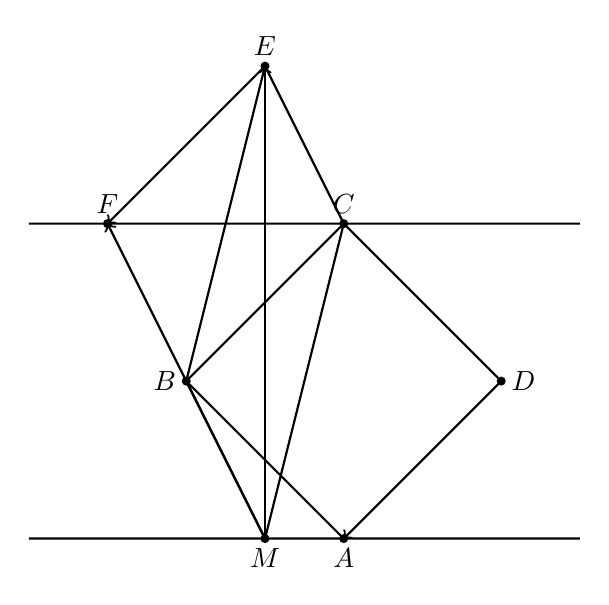
\begin{tikzpicture}[thick]
				\coordinate (A) at (1,0);\coordinate (B) at (-1,2);\coordinate (C) at (1,4); 
				\coordinate (D) at (3,2);\coordinate (M) at (0,0); \coordinate (E) at (0,6);
				\coordinate (F) at (-2,4);  
				\draw (A)--(B)--(C)--(D)  (M)--(B)--(E)--(C)--cycle  (-3,0)--(4,0) (-3,4)--(4,4);  
				\draw[->] (M)--(F);\draw[->] (M)--(E);\draw[->] (D)--(A); \draw[->] (E)--(F); 
				\foreach\i in {M,A}\draw[fill] (\i) circle (1.2pt) node[below] {$\i$} ;
				\foreach\i in {C,E,F}\draw[fill] (\i) circle (1.2pt) node[above] {$\i$} ;
				\draw[fill] (B) circle (1.2pt) node[left] {$B$} ;
				\draw[fill] (D) circle (1.2pt) node[right] {$D$} ;
			\end{tikzpicture}
		\end{center}
		Dựng hình bình hành $MBEC$, $BCEF$,  ta có $|\overrightarrow{MA}+\overrightarrow{MB}+\overrightarrow{MC} -\overrightarrow{MD}|=|\overrightarrow{ME}+\overrightarrow{DA}|=|\overrightarrow{ME}+\overrightarrow{EF}| =|\overrightarrow{MF}|$. Khi $M$ thay đổi trên $d$ thì $F$ thuộc đường thẳng cố định 
		qua $C$ song  song với $d$, điểm $M$ cần tìm là hình chiếu vuông góc của $B$ trên $d$.\\
		Khi đó, ta có $|\overrightarrow{MD}|=MD=\sqrt{BD^2+BM^2}=\dfrac{a\sqrt{10}}{2}$. 
	}
\end{ex}
%%==========Câu 3
\begin{ex}
	\immini
	{
		Cho hai lực $\overrightarrow{F}_{1}=\overrightarrow{M A}$,  $\overrightarrow{F}_{2}=\overrightarrow{M B}$ cùng tác động vào một vật tại điểm $M$ cường độ hai lực $\overrightarrow{F}_{1}$, $\overrightarrow{F}_{2}$ đều bằng $300$ (N) và $\widehat{AMB}=120^{\circ}$. Tìm cường độ của lực tổng hợp tác động vào vật.
		\choice
		{\True $300$ (N)}
		{$700$ (N)}
		{$100$ (N)}
		{$500$ (N)}	
	}
	{
		\begin{tikzpicture}[>=stealth,line join=round,line cap=round,font=\footnotesize,scale=0.8]
			\path (0,0) coordinate (M)
			(3,0) coordinate (A)
			(120:3) coordinate (B)
			;
			\draw[->] (M)--(A);
			\draw[->] (M)--(B);
			% \tkzMarkAngles[arc=ll,mark={}](A,M,B)
			% \draw (M) node[below right]{$120^\circ$};
			\foreach \p/\r in {A/90,M/180,B/0}
			\draw (\p)  node[shift={(\r:3mm)}]{$\p$};
	\end{tikzpicture}	}
	\loigiai{
		\immini
		{
			Gọi $D$ là đỉnh thứ tư của hình thoi $MBDA$, ta có 
			$$\overrightarrow{MA}+\overrightarrow{MB}=\overrightarrow{MD}.$$
			Vậy cường độ lực tổng hợp tại $M$ là 
			$\left|\overrightarrow{MD}\right|=MD$.
		}
		{
			\begin{tikzpicture}[>=stealth,line join=round,line cap=round,font=\footnotesize,scale=0.8]
				\path (0,0) coordinate (M)
				(3,0) coordinate (A)
				(120:3) coordinate (B)
				($(B)+(A)-(M)$) coordinate (D)
				($(B)!1/2!(A)$) coordinate (O)
				;
				\draw[->] (M)--(A);
				\draw[->] (M)--(B);
				\draw[->] (M)--(D);
				\draw[dashed] (B)--(D)--(A) (B)--(A);
				% \tkzMarkAngles[size=0.5cm,arc=ll,mark={}](M,B,D)
				% \draw (B) node[above right=0.2, rotate=5]{$60^\circ$};
				\foreach \p/\r in {A/0,M/180,B/90,D/90,O/0}
				\draw (\p)  node[shift={(\r:3mm)}]{$\p$};
			\end{tikzpicture}	
		}
		\noindent 
		Gọi $O$ là tâm hình thoi $MBDA$ có cạnh $300$, do $\widehat{BMA}=120^\circ \Rightarrow \widehat{ MBD}=60^\circ$.
		\\
		Vậy tam giác $MBD$ đều cạnh $300$ suy ra $MD=300$ (N).		
	}
\end{ex}


%%==========Câu 4
\begin{ex}
	\immini
	{
		Cho ba lực $\overrightarrow{F}_{1}=\overrightarrow{M A}$, $ \overrightarrow{F}_{2}=\overrightarrow{M B}$,  $\overrightarrow{F}_{3}=\overrightarrow{M C}$ cùng tác động vào một vật tại điểm $M$ và vật đứng yên. Cho biết cường độ của $\overrightarrow{F}_{1}$, $\overrightarrow{F}_{2}$ đều bằng $25$ (N) và góc $\widehat{AMB}=60^{\circ}.$ Khi đó cường độ lực của $\overrightarrow{F}_{3}$ là	
	}
	{
		\begin{tikzpicture}[>=stealth,line join=round,line cap=round,font=\footnotesize,scale=1]
			\path (0,0) coordinate (M)
			(-30:2) coordinate (B)
			(30:2) coordinate (A)
			(-3,0) coordinate (C) 
			;
			\draw[->] (M)--(C); 
			\draw[->] (M)--(A); 
			\draw[->] (M)--(B); 
			% \tkzMarkAngles[size=1cm,arc=ll,mark={}](B,M,A)
			% \draw (M) node[right=0.3]{$60^\circ$};
			\foreach \p/\r in {M/90,A/60,B/-60,C/90}
			\fill (\p)  node[shift={(\r:3mm)}]{$\p$};
		\end{tikzpicture}	
	}
	\choice
	{\True $25 \sqrt{3} $ (N)}
	{$50 \sqrt{3}$ (N)}
	{$50 \sqrt{2}$ (N)}
	{$100 \sqrt{3}$ (N)}
	\loigiai{
		\immini
		{
			Gọi $D$ là đỉnh thứ tư của hình thoi $MADB$, ta có 
			$$\overrightarrow{MA}+\overrightarrow{MB}=\overrightarrow{MD}.$$
			Vậy lực tổng hợp tại $M$ là 
			$$\overrightarrow{MA}+\overrightarrow{MB}+\overrightarrow{MC}=\overrightarrow{MD}+\overrightarrow{MC}.$$
		}
		{
			\begin{tikzpicture}[>=stealth,line join=round,line cap=round,font=\footnotesize,scale=1]
				\path (0,0) coordinate (M)
				(-30:2) coordinate (B)
				(30:2) coordinate (A)
				(-3,0) coordinate (C) 
				(3.464101615,0) coordinate (D)
				(2,0) coordinate (O)
				;
				\draw[->] (M)--(C); 
				\draw[->] (M)--(A); 
				\draw[->] (M)--(B);
				\draw[->] (M)--(D);
				\draw (A)--(D)--(B); 
				\draw (A)--(B);
				% \tkzMarkAngles[size=1cm,arc=ll,mark={}](B,M,A)
				% \draw (M) node[above right=0.3,rotate=20]{$60^\circ$};
				\foreach \p/\r in {M/90,A/60,B/-60,C/90,O/80,D/0}
				\fill (\p)  node[shift={(\r:3mm)}]{$\p$};
			\end{tikzpicture}		
		}
		\noindent Do vật đứng yên nên $\overrightarrow{MD}+\overrightarrow{MC}=\overrightarrow{0}\Rightarrow \overrightarrow{MC}=-\overrightarrow{MD}$.
		\\
		Vậy cường độ lực $\overrightarrow{F}_3$ là 
		$$ \left|\overrightarrow{MC}\right|=\left|\overrightarrow{MD}\right|=MD.$$
		Gọi $O$ là tâm hình thoi $MBDA$ có cạnh $25$, ta có 
		$MD=2MO=25 \sqrt 3$ (N).	
	}
\end{ex}




%%==========Câu 3
\begin{ex}
	\immini
	{
		Cho ba lực $\overrightarrow{F}_{1}=\overrightarrow{M A}$,  $\overrightarrow{F}_{2}=\overrightarrow{M B}$, $\overrightarrow{F}_{3}=\overrightarrow{M C}$ cùng tác động vào một vật tại điểm $M$ cường độ hai lực $\overrightarrow{F}_{1}$, $\overrightarrow{F}_{2}$ đều bằng $300$ (N) và $\overrightarrow{F}_{3}=400$ (N). Lại có $\widehat{AMB}=120^{\circ}$ và $\widehat{AMC}=60^{\circ}$. Tìm cường độ của lực tổng hợp tác động vào vật.
		\choice
		{$300$ (N)}
		{\True $700$ (N)}
		{$100$ (N)}
		{$500$ (N)}	
	}
	{
		\begin{tikzpicture}[>=stealth,line join=round,line cap=round,font=\footnotesize,scale=0.8]
			\path (0,0) coordinate (M)
			(3,0) coordinate (A)
			(120:3) coordinate (B)
			(60:4) coordinate (C)
			;
			\draw[->] (M)--(A);
			\draw[->] (M)--(B);
			\draw[->] (M)--(C);
			% \tkzMarkAngles[arc=ll,mark={}](A,M,B)
			% \tkzMarkAngles[size=0.5cm,arc=ll,mark={}](A,M,C)
			% \draw (M) node[above left]{$120^\circ$};
			% \draw (M) node[below right]{$60^\circ$};
			\foreach \p/\r in {A/90,M/180,B/0,C/60}
			\draw (\p)  node[shift={(\r:3mm)}]{$\p$};
	\end{tikzpicture}	}
	\loigiai{
		\immini
		{
			Gọi $D$ là đỉnh thứ tư của hình thoi $MBDA$, ta có 
			$$\overrightarrow{MA}+\overrightarrow{MB}=\overrightarrow{MD}.$$
			Vậy cường độ lực tổng hợp tại $M$ là $$\left|\overrightarrow{MA}+\overrightarrow{MB}+\overrightarrow{MC}\right|=\left|\overrightarrow{MD}+\overrightarrow{MC}\right|.$$
		}
		{
			\begin{tikzpicture}[>=stealth,line join=round,line cap=round,font=\footnotesize,scale=0.8]
				\path (0,0) coordinate (M)
				(3,0) coordinate (A)
				(120:3) coordinate (B)
				(60:4) coordinate (C)
				($(A)!1/2!(B)$) coordinate (O)
				($(A)+(B)-(M)$) coordinate (D)
				;
				\draw[->] (M)--(A);
				\draw[->] (M)--(B);
				\draw[->] (M)--(C);
				\draw[->] (M)--(D);
				\draw[dashed] (B)--(D)--(A)--(B);
				% \tkzMarkAngles[arc=ll,mark={}](A,M,B)
				% \tkzMarkAngles[size=0.5cm,arc=ll,mark={}](A,M,C)
				% \draw (M) node[above left]{$120^\circ$};
				% \draw (M) node[below right]{$60^\circ$};
				\foreach \p/\r in {A/00,M/-160,B/90,C/60,D/90,O/100}
				\draw (\p)  node[shift={(\r:3mm)}]{$\p$};
			\end{tikzpicture}	
		}
		\noindent  Lại có $\overrightarrow{MD}$ và $\overrightarrow{MD}$ là $2$ vectơ cùng hướng nên 
		$\left|\overrightarrow{MD}+\overrightarrow{MC}\right|=MD+MC$.
		\\
		Gọi $O$ là tâm hình thoi $MBDA$ có cạnh $300$, do $\widehat{BMA}=120^\circ \Rightarrow \widehat{ MBD}=60^\circ$.
		\\
		Vậy tam giác $MBD$ đều cạnh $300$ suy ra $MD=300$ (N).	
		\\
		Vậy cường độ lực tổng hợp tại $M$ là $MD+MC=300+400=700$ (N).	
	}
\end{ex}


%%==========Câu 3
\begin{ex}
	\immini
	{
		Cho ba lực $\overrightarrow{F}_{1}=\overrightarrow{M A}$,  $\overrightarrow{F}_{2}=\overrightarrow{M B}$, $\overrightarrow{F}_{3}=\overrightarrow{M C}$ cùng tác động vào một vật tại điểm $M$ cường độ hai lực $\overrightarrow{F}_{1}$, $\overrightarrow{F}_{2}$ đều bằng $300$ (N) và $\overrightarrow{F}_{3}=400$ (N). Lại có $\widehat{AMB}=120^{\circ}$ và $\widehat{AMC}=150^{\circ}$. Tìm cường độ của lực tổng hợp tác động vào vật.
		\choice
		{$300$ (N)}
		{\True $700$ (N)}
		{$100$ (N)}
		{$500$ (N)}	
	}
	{
		\begin{tikzpicture}[>=stealth,line join=round,line cap=round,font=\footnotesize,scale=0.8]
			\path (0,0) coordinate (M)
			(3,0) coordinate (A)
			(120:3) coordinate (B)
			(150:4) coordinate (C)
			;
			\draw[->] (M)--(A);
			\draw[->] (M)--(B);
			\draw[->] (M)--(C);
			% \tkzMarkAngles[size=0.5cm,arc=ll,mark={}](A,M,B)
			% \tkzMarkAngles[size=0.3cm,arc=ll,mark={}](A,M,C)
			% \draw (M) node[above right=0.2]{$120^\circ$};
			% \draw (M) node[below]{$150^\circ$};
			\foreach \p/\r in {A/90,M/180,B/0,C/60}
			\draw (\p)  node[shift={(\r:3mm)}]{$\p$};
	\end{tikzpicture}	}
	\loigiai{
		\immini
		{
			Gọi $D$ là đỉnh thứ tư của hình thoi $MBDA$, ta có 
			$$\overrightarrow{MA}+\overrightarrow{MB}=\overrightarrow{MD}.$$
			Vậy cường độ lực tổng hợp tại $M$ là $$\left|\overrightarrow{MA}+\overrightarrow{MB}+\overrightarrow{MC}\right|=\left|\overrightarrow{MD}+\overrightarrow{MC}\right|.$$
		}
		{
			\begin{tikzpicture}[>=stealth,line join=round,line cap=round,font=\footnotesize,scale=0.8]
				\path (0,0) coordinate (M)
				(3,0) coordinate (A)
				(120:3) coordinate (B)
				(150:4) coordinate (C)
				(60:3) coordinate (D)
				($(B)!1/2!(A)$) coordinate (O)
				;
				\draw[->] (M)--(A);
				\draw[->] (M)--(B);
				\draw[->] (M)--(C);
				\draw[->] (M)--(D);
				\draw[dashed] (B)--(D)--(A)--(B);
				% \tkzMarkAngles[size=0.5cm,arc=ll,mark={}](A,M,B)
				% \tkzMarkAngles[size=0.3cm,arc=ll,mark={}](A,M,C)
				% \draw (M) node[above right=0.2]{$120^\circ$};
				% \draw (M) node[below]{$150^\circ$};
				
				% \tkzMarkRightAngles[size=0.5](D,M,C) % Đánh dấu nhiều góc vuông
				\foreach \p/\r in {A/0,M/180,B/90,C/60,D/60,O/90}
				\draw (\p)  node[shift={(\r:3mm)}]{$\p$};
			\end{tikzpicture}	
		}
		\noindent  
		Gọi $O$ là tâm hình thoi $MBDA$ có cạnh $300$, do $\widehat{BMA}=120^\circ \Rightarrow \widehat{ MBD}=60^\circ$.
		\\
		Vậy tam giác $MBD$ đều cạnh $300$ suy ra $MD=300$ (N) và $\widehat{DMA}=60^\circ$. 
		\\
		Suy ra	
		$\widehat{CMD}=150^\circ -60^\circ = 90^\circ$ hay tam giác $CMD$ vuông tại $M$.
		\immini
		{
			Gọi $E$ là đỉnh thứ tư của hình chữ nhật $CMDE$, ta có 
			$$\left|\overrightarrow{MD}+\overrightarrow{MC}\right|=\left|\overrightarrow{ME}\right|=ME.$$
			Do $CMDE$ là hình chữ nhật nên $$ME=\sqrt{300^2+400^2}=500~	\mathrm{(N)}.$$
		}
		{
			\begin{tikzpicture}[>=stealth,line join=round,line cap=round,font=\footnotesize,scale=0.7]
				\path (0,0) coordinate (M)
				(3,0) coordinate (A)
				(120:3) coordinate (B)
				(150:4) coordinate (C)
				(60:3) coordinate (D)
				($(B)!1/2!(A)$) coordinate (O)
				($(C)+(D)-(M)$) coordinate (E)
				;
				\draw[->] (M)--(A);
				\draw[->] (M)--(B);
				\draw[->] (M)--(C);
				\draw[->] (M)--(D);
				\draw[->] (M)--(E);
				\draw[dashed] (B)--(D)--(A)--(B) (C)--(E)--(D);
				%			\tkzMarkAngles[size=0.5cm,arc=ll,mark={}](A,M,B)
				%			\tkzMarkAngles[size=0.3cm,arc=ll,mark={}](A,M,C)
				%			\draw (M) node[above right=0.2]{$120^\circ$};
				%			\draw (M) node[below]{$150^\circ$};
				
				\tkzMarkRightAngles[size=0.5](D,M,C) % Đánh dấu nhiều góc vuông
				\foreach \p/\r in {A/0,M/180,B/90,C/60,D/60,O/90,E/90}
				\draw (\p)  node[shift={(\r:3mm)}]{$\p$};
			\end{tikzpicture}
		}	
	}
\end{ex}
\Closesolutionfile{ans}
\Closesolutionfile{ansbook}
% % \indapan{10}{ans/ans-0H1-8-TN}